\chapter{Deep Learning Overview}\label{chap:dlo}

\localtableofcontents

\section{Introduction}

Deep Learning is a subfield of machine learning that focuses on the study of
\acfp{DNN} which have their roots in \acfp{ANN}. \acp{DNN} aim to learn a
representation from unstructured data such as raw images
\cite{DBLP:conf/nips/KrizhevskySH12}, text
\cite{DBLP:conf/emnlp/BudzianowskiV19} or audio
\cite{DBLP:journals/corr/HannunCCCDEPSSCN14}, in an end-to-end fashion.
\acp{DNN} have been used to solve a wide range of tasks, including image and
speech recognition
\cite{DBLP:conf/nips/KrizhevskySH12,DBLP:journals/corr/SimonyanZ14a,DBLP:conf/cvpr/HeZRS16,DBLP:journals/corr/HannunCCCDEPSSCN14,DBLP:conf/icassp/ChanJLV16,DBLP:conf/icml/AmodeiABCCCCCCD16},
natural language processing
\cite{DBLP:conf/emnlp/BudzianowskiV19,DBLP:conf/naacl/DevlinCLT19,DBLP:conf/nips/VaswaniSPUJGKP17},
object detection \cite{DBLP:conf/cvpr/RedmonDGF16,DBLP:conf/nips/RenHGS15},
semantic segmentation \cite{long2015fully,DBLP:conf/cvpr/LiuCSAHY019}, text and
image generation
\cite{goodfellow2020generative,karras2019style,DBLP:conf/emnlp/BudzianowskiV19}
as well as exotic domains like video games
\cite{silver2016mastering,silver2018general} or molecules folding
\cite{jumper2021highly}. \acp{ANN} were initially conceptualised based on the
understanding of biological neural networks present in the brain
\cite{mcculloch1943logical,hebb2005organization}.
\citeauthor{rosenblatt1958perceptron} proposed in
\cite{rosenblatt1958perceptron} a theoretical model of a neuron, denoted the
\emph{perceptron}, which was capable of learning a linear decision boundary. The
perceptron model was later extended to multiple layers of neurons, giving rise
to the \acf{MLP} \cite{rosenblatt1961principles,rumelhart1986learning}. A
\acl{MLP} is a type of artificial neural network that extends the concept of a
single-layer perceptron by including one or more hidden layers of neurons
connected downstream from an input layer and upstream to an output layer. Each
layer is fully connected to the next, allowing the model to learn and represent
more complex, non-linear relationships in the input data. Although more capable
than the perceptron, the \ac{MLP} is still limited by its depth. The next
advance came from the stacking of multiple layers, leading to \aclp{DNN}.\\

In the context of \acp{DNN}, the term \emph{deep} denotes the stacking of many
layers within a neural network. The concept of \acp{DNN} is based on the idea
that the depth and the numerous layers can help in learning features at various
levels of abstraction, enabling the network to learn complex hierarchical
pattern representations. For instance, in the context of image recognition, lower layers learn
local features like edges and textures, while deeper layers learn to identify
more abstract concepts like shapes or objects.\\

The rise of \acp{DNN} was made possible by several factors. On the one hand the
increase in computational power, and in particular the use of \acp{GPU}, made
the training of large and deep networks feasible. Indeed, AlexNet, the first
\ac{CNN} to win the ImageNet Large Scale Visual Recognition Challenge
\cite{DBLP:conf/nips/KrizhevskySH12}, was trained on two \acp{GPU} in parallel
to accelerate computations. Nowadays, the use of \acp{GPU} or dedicated hardware
such as \acp{TPU} \cite{jouppi2017datacenter} is ubiquitous and supported by all
the major deep learning frameworks
\cite{DBLP:journals/corr/AbadiABBCCCDDDG16,DBLP:conf/nips/PaszkeGMLBCKLGA19}. On
the other hand, the availability of large-scale datasets such as ImageNet
\cite{deng2009imagenet} allowed to train or pre-train deep networks with
millions of parameters without overfitting.\\

This chapter aims to give an overview of the different neural network
architectures, building blocks, training techniques and datasets that are widely
used in Deep Learning for computer vision and in our experiments.
\Cref{sec:dlo:early_architectures} introduces the early neural network
architectures, namely the perceptron and the \ac{MLP}. \Cref{sec:dlo:training}
focuses on the functional definition of a neural network and its training.
\Cref{sec:dlo:cnn} presents the building blocks and architectures of various
\acp{CNN} for computer vision, and in particular the ones we benchmark our
methods with (see \cref{sec:chap1:experiments,sec:chap2:experiments}). Finally,
\Cref{sec:dlo:datasets} gives an overview of the most prevalent datasets that we
used in our experiments.


\section{Early Architectures}\label{sec:dlo:early_architectures}

In this section, we present the perceptron \cite{rosenblatt1958perceptron} and
then the \acl{MLP} \cite{rosenblatt1961principles,rumelhart1986learning}. Both
are the two founding neural network architectures that led to the development of
\aclp{DNN}.

\subsection{Perceptron}\label{sec:dlo:perceptron}

The \emph{perceptron} is a model of artificial neuron, capable of learning a
linear decision boundary. It was proposed by
\citeauthor{rosenblatt1958perceptron} in 1958 \cite{rosenblatt1958perceptron}
and conceptualised based on the understanding of biological neural networks
present in the brain \cite{mcculloch1943logical,hebb2005organization}. The
perceptron is composed of inputs that are weighted and summed before being
passed through a nonlinear function referred to as an activation function. The
conceptual representation of the perceptron is displayed in
\cref{fig:dlo:perceptron} and its mathematical formulation is defined in
\cref{eqn:dlo:perceptron}: \\
% and can be express in vector form as written in \cref{eqn:dlo:perceptron_vector}.\\

\begin{equation}
  \label{eqn:dlo:perceptron}
\hat{y} = g(\sum_{i=1}^{n} w_i \cdot x_i + b)
\end{equation} \\


% \begin{equation}
%   \label{eqn:dlo:perceptron_vector}
%   \hat{y} = g(\mathbf{w}^T \mathbf{x} + b)
% \end{equation}\\

\noindent where $x_i$ is the $i$th input, $w_i$ its associated weight, $n$ is
the number of inputs, $b$ is the bias, $g$ is the activation function, and
$\hat{y}$ is the output of the perceptron. This formulation can also be written
in vector form as in \cref{eqn:dlo:perceptron_vector}: \\

\begin{equation}
  \label{eqn:dlo:perceptron_vector}
  \hat{y} = g(\mathbf{w}^T \mathbf{x} + b)
\end{equation}\\

\noindent where $\mathbf{x}$ is the vector of inputs and $\mathbf{w}$ is the
vector of weights. The activation function $g$ is typically a nonlinear
function, such as the sigmoid or the hyperbolic tangent (see
\cref{fig:dlo:activation_functions}). Due to its shallow architecture, the
perceptron cannot learn complex decision boundaries. Nevertheless, it is
possible to stack several perceptrons to learn nonlinear decision boundaries,
leading to a \acl{MLP}.\\

\begin{figure}[htbp]
  \centering
  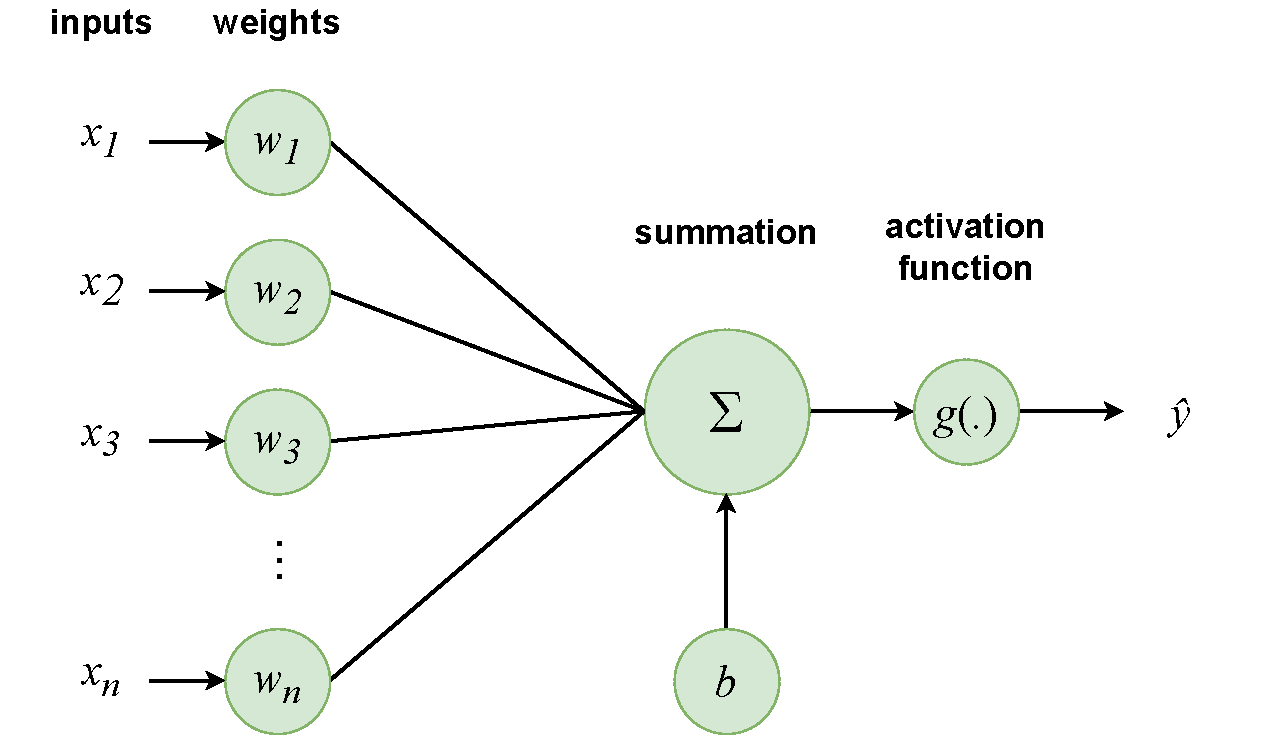
\includegraphics[width=0.7\textwidth]{chapter_dlo/assets/perceptron_scheme.pdf}
  \caption{Conceptual scheme of the \emph{perceptron}. Each input $x_i$ is multiplied
  by its associated weight $w_i$ and summed to the other weighted inputs. The
  bias $b$ is added to the sum and the result is passed through an activation
  function $g$ to produce the output $\hat{y}$.}
  \label{fig:dlo:perceptron}
\end{figure}

\subsection{Multilayer Perceptron}\label{sec:dlo:mlp}

The \acf{MLP} is an extension of the perceptron model, comprising multiple
layers of perceptrons, also referred to as neurons \cite{rumelhart1986learning}.
A \ac{MLP} with one hidden layer is represented in \cref{fig:dlo:mlp}. In the
latter, the circles represent the neurons and the connections between them,
representing weights, are materialised by lines. The \ac{MLP} is the simplest
type of feedforward \ac{ANN}. Feedforward refers to the fact that the
connections between neurons in the \ac{MLP} form a directed acyclic graph, where
the outputs of the neurons from one layer are passed to the next, with no
backward connections or feedback. Using the same notations as in
\cref{eqn:dlo:perceptron_vector}, the vector form of the \ac{MLP} displayed in
\cref{fig:dlo:mlp} can be written as in \cref{eqn:dlo:mlp}, where the subscript
of activation functions $g_i$, weight matrices $\mathbf{w}_i$ and bias vectors
$\mathbf{b}_i$ denotes their belonging to the $i$th layer.\\

\begin{equation}
  \label{eqn:dlo:mlp}
  \hat{\mathbf{y}} = g_2(\mathbf{w}_2^T \cdot  g_1(\mathbf{w}_1^T \cdot \mathbf{x} + \mathbf{b}_1) + \mathbf{b}_2)
\end{equation}\\

Each layer of the \ac{MLP}, being fully connected to the next one, enables the
\ac{MLP} to handle problems that the perceptron cannot solve, such as problems
requiring nonlinear decision boundaries. Furthermore,
\citeauthor{cybenko1989approximation} proved in \cite{cybenko1989approximation}
that an \ac{MLP} can approximate continuous functions on compact subsets of
$\mathds{R}^n$. This result is known as the \emph{Universal Approximation
Theorem}. Before the emergence of Deep Learning, \acp{MLP} have been applied to
various domains, including voice recognition, image recognition, and machine
translation \cite{wasserman1988neural}.


\begin{figure}[htbp]
  \centering
  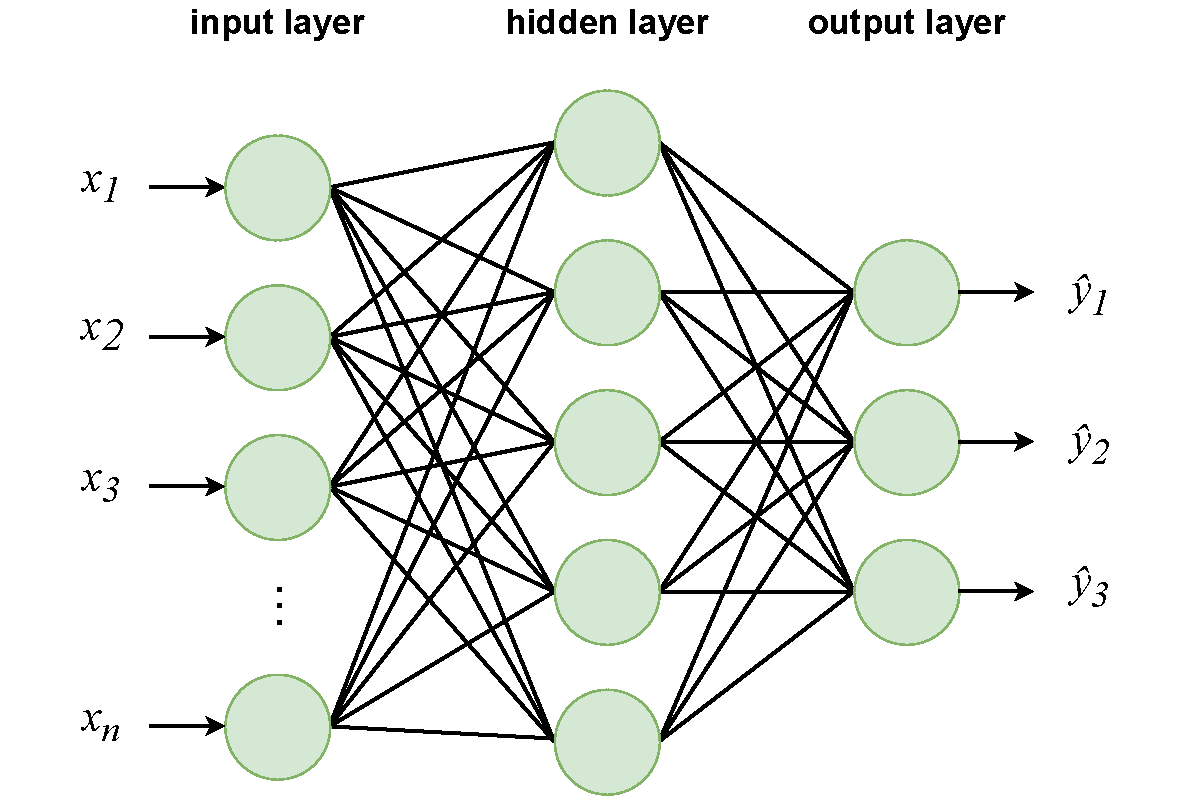
\includegraphics[width=0.7\textwidth]{chapter_dlo/assets/mlp_scheme.pdf}
  \caption{Conceptual scheme of a \ac{MLP} with one hidden layer. Each circle
  represents a neuron and each line a connection associated with a weight.}
  \label{fig:dlo:mlp}
\end{figure}

\section{Neural Network Training}\label{sec:dlo:training}

Neural Network Training revolves around the optimisation of a mapping function
that learns to predict an output given input data by adjusting its internal
parameters, also referred to as weights. This optimisation, also called
\emph{training}, involves iteratively tuning these weights so that the
discrepancy between the output predicted by the model and the reference output
is minimised. Weights tuning relies on gradient-based methods that hinge
around two core components: the \emph{backpropagation} algorithm to compute the
gradients and the \ac{SGD} algorithm to update the weights.

\subsection{Functional Definition}

Neural networks can be defined as a mapping function from an input space
$\mathcal{X}$ to an ouput space $\mathcal{Y}$. This mapping function $f$ is
characterised by a set of parameters $\theta$, often called \emph{weights}. The
training of a neural network consists in tuning the parameters $\theta$ so that,
given an input $X$, the mapping function $f$ output, denoted $\hat{y}$, is as
close as possible to the associated true output $y$. This training is done
iteratively by using example pairs $(X, y) \in \mathcal{X} \times \mathcal{Y}$,
where $X\in\mathcal{X}$ is the input and $y\in\mathcal{Y}$ is the output. In the
context of image classification, $X$ is an image and $y$ is a label that
indicates the class of the associated image. A functional representation of a
neural network is given in \cref{eqn:dlo:nn_functional_definition}, where $f$ is
the neural network, $\theta$ is the set of parameters of the network,
$X\in\mathcal{X}$ is the input given to the neural network and $\hat{y}$ is the
output.\\

\begin{equation}
  \label{eqn:dlo:nn_functional_definition}
  % \centering
  \begingroup
  \setlength\arraycolsep{0pt}
  f \colon\begin{array}[t]{c >{{}}c<{{}} l}
    \mathcal{X} & \to     & \mathcal{Y} \\
    X                     & \mapsto & f(X, \theta) = \hat{y}
  \end{array}
  \endgroup
\end{equation}\\


Considering image classification,  the output $\hat{y}$ is a probability vector
where the largest coefficient is the one whose index corresponds to the
predicted class of the input image. This vector is generally converted into a
one-hot vector, where the only non-zero coefficient is at the index of the
predicted class. The true label $y$, referred to as the ground truth, is the
class index so that $y\in\llbracket0;C-1\rrbracket$, where $C$ is the number of
classes considered. The ground truth can also be converted into a one-hot
vector.\\

% In the case of image classification, the input $X$ given to the neural network
% is an image, and the output $\hat{y}$ is a probability vector where the largest
% coefficient is the one whose index corresponds to the predicted class of the
% input image. $y_i$, often referred to as the ground truth is a one-hot vector
% where the only non-zero coefficient is at the index corresponding to the true
% class of the input image.\\

% A neural network is a function that maps an input $X$ to an output $y$ through
% a series of transformations. The functional definition of a neural network is
% given in \cref{eqn:dlo:nn_functional_definition}, where $f$ is the neural
% network, $\theta$ is the set of parameters of the network, and $y$ is the
% output.\\

\subsection{Loss Function and Regularisation}
Training a neural network aims at finding the optimal parameters $\theta$ that
maximise a performance, quantified by a metric, often based on the discrepancy
between the predicted output $\hat{y}$ and the true output $y$. However,
optimising directly the metric might be intractable. To solve this issue, one
may define a differentiable cost function and minimise the latter as a proxy for
optimising the metric. Considering $k$ example pairs $(X_k, y_k)$, the cost
function $\mathcal{J}(\theta)$, also referred to as the
\emph{empirical risk}, is defined in the following equation:

\begin{equation}
  \label{eqn:dlo:cost_function}
  % \mathcal{J}_\text{emp}(\theta) = \mathds{E}_{(X, y) \sim \delta} \left[ \mathcal{L}(f(X,\theta), y) \right]
  \mathcal{J}(\theta) = \frac{1}{k} \sum_{i=1}^{k} \mathcal{L}(f(X_k,\theta), y_k)
\end{equation}\\

\noindent where $\mathcal{L}$ is the loss function. Note that the true data
distribution, and therefore the risk, is unknown. This is why the empirical
risk, computed with a set of example pairs, is used instead. The minimisation of
the empirical risk alone is not sufficient to ensure good overall performance.
Indeed, the neural network could learn to perfectly predict the output of the
training set but may fail to generalise to unseen data. This phenomenon is
called \emph{overfitting}. To prevent overfitting, we add a regularisation term
to the empirical risk. The regularisation term, denoted $\mathcal{R}$, is a
function of the parameters $\theta$ of the neural network which penalises the
complexity of the model, and thus prevents overfitting. To account for
regularisation, the cost function in \cref{eqn:dlo:cost_function} is updated to:

\begin{equation}
  \label{eqn:dlo:regularised_cost_fn}
  % \mathcal{J}_r(\theta) = \mathds{E}_{(X, y) \sim \delta} \left[ \mathcal{L}(f(X,\theta), y) \right] + \mathcal{R}(\theta) 
  \mathcal{J}_r(\theta) =   \frac{1}{k} \sum_{i=1}^{k} \mathcal{L}(f(X,\theta), y) + \mathcal{R}(\theta) 
\end{equation}\\

\noindent\textbf{Loss function.} In
\cref{eqn:dlo:cost_function,eqn:dlo:regularised_cost_fn}, the loss function
$\mathcal{L}$ is a measure of the discrepancy between the ground truth $y$ and
the predicted output. Contrary to the metric $P$ which might be
non-differentiable, the loss function is differentiable so that its minimisation
can be achieved using gradient-based methods, subsequently detailed in
\cref{sec:dlo:backpropagation}. The choice of the loss function depends on the
task at hand. For classification tasks (not only images), the loss function is
often the \emph{cross-entropy} loss. For a binary classification problem, the
ground truth is a binary variable $y\in \{0,1\}$ and the predicted output is a
scalar $f(X,\theta)=\hat{y}\in[0,1]$. The binary cross-entropy loss is defined
as follows:\\

\begin{equation}
  \label{eqn:dlo:binary_cross_entropy_loss}
  \mathcal{L}(\hat{y}, y) = - y \log(\hat{y}) - (1-y) \log(1-\hat{y})
\end{equation}\\

\noindent The binary cross-entropy loss defined in
\cref{eqn:dlo:binary_cross_entropy_loss} can be extended to problems with more
than two classes. For a classification problem with $C$ classes, the ground
truth is a one-hot vector $\mathbf{y}\in \{0,1\}^C$ and the output is a
$C$-dimensional vector $f(X,\theta)=\hat{\mathbf{y}}\in\mathds{R}^C$. The
multi-class cross-entropy loss is defined as follows:

\begin{equation}
  \label{eqn:dlo:multiclass_cross_entropy_loss}
  % \mathcal{L}(\hat{\mathbf{y}}, \mathbf{y}) = - \sum_{i=1}^c y_i \log \left( \displaystyle\frac{\exp(\hat{y}_i)}{\displaystyle\sum_{j=1}^c \exp(\hat{y}_j)} \right)
  \mathcal{L}(\hat{\mathbf{y}}, \mathbf{y}) = - \sum_{i=1}^C y_i \log \left( \phi(\mathbf{\hat{y}})_i \right)
\end{equation}\\


\noindent In the above equation, $\hat{\mathbf{y}}$ is the unnormalised raw
output vector of the neural network and $\phi$ is the softmax function, whose
expression is given in \cref{eqn:dlo:softmax}. The softmax function is used to
convert the raw output vector of real numbers into a probability distribution.
Note that some models which use the softmax as the activation function of their
last layer output directly a probability distribution, in which case the softmax
is not needed.\\

Considering a vector $\mathbf{z} = [z_1, \dots, z_n]$, the $j$-th component of
vector $\mathbf{z}$ normalised by the softmax function is given by: 

\begin{equation}
  \label{eqn:dlo:softmax}
  % \phi(\mathbf{z})_j = \frac{\exp(z_j)}{\displaystyle\sum_{k=1}^{\text{dim}(\mathbf{z})} \exp(z_k)}
  \phi(\mathbf{z})_j = \frac{\exp(z_j)}{\displaystyle\sum_{k=1}^{n} \exp(z_k)}
\end{equation}\\

\noindent \textbf{Regularisation.} The regularisation term $\mathcal{R}$ is a
differentiable function of the weights $\theta$. It acts as a control mechanism
to avoid overfitting by preventing the weights of the neural network from
becoming too large, which can lead to overly complex models that overfit the
training data. This is typically achieved by adding a penalty proportional to
the magnitude of the weights, thereby keeping them small.\\

Common types of regularisation include $\ell_1$ and $\ell_2$ regularisation,
whose expressions are shown in \cref{eqn:dlo:reg_l1,eqn:dlo:reg_l2}
respectively. $\ell_1$ regularisation \cite{tibshirani1996regression}, adds a
penalty equal to the absolute value of the magnitude of the weights. On the
other hand, $\ell_2$ regularisation \cite{hoerl1970ridge}, adds a penalty
equivalent to the square of the magnitude of the weights. Both methods aim to
reduce the magnitude of the weights, but $\ell_1$ regularisation is more
targeted towards feature selection, effectively pushing some weights to $0$,
whereas $\ell_2$ restrains globally their magnitude.\\

The regularisation term $\mathcal{R}$ is added to the cost function with a
regularisation coefficient, usually denoted as $\lambda$, which is a
hyperparameter that balances the trade-off between fitting the training data
(minimising the loss $\mathcal{L}$) and limiting the complexity of the model
(minimising $\mathcal{R}$).\\

For a network with L layers and parameters $\theta=\{\mathbf{w}_1, \dots,
\mathbf{w}_L\}$, the $\ell_1$ and $\ell_2$ regularisation term is defined as
follows:\\

\begin{equation}
  \label{eqn:dlo:reg_l1}
  \mathcal{R}_{\ell_1}(\theta) = \lambda \sum_{i=1}^{L} \| \mathbf{w}_i \|_1
\end{equation}\\

\begin{equation}
  \label{eqn:dlo:reg_l2}
  \mathcal{R}_{\ell_2}(\theta) = \frac{\lambda}{2} \displaystyle \sum_{i=1}^{L} \| \mathbf{w}_i \|_2^2 
\end{equation}\\

\noindent where $\|. \|_1$ and $\|.\|_2^2$ respectively denote the sum of
the absolute value and the sum of the squaring of each element of the vector.\\

\subsection{Loss Optimisation}\label{sec:dlo:backpropagation}

As mentioned before, the training of a neural network involves finding the
optimal set of parameters $\theta$ that minimises a cost function
$\mathcal{J}(\theta)$. This process of optimisation is typically carried out
using gradient-based methods which rely on the iterative adjustment of the
parameters in the opposite direction of the gradient of the cost function. The
gradient of a function provides the direction of the steepest ascent at a given
point \cite{boyd2004convex}. Thus, by moving the parameters in the opposite
direction of the gradient, we seek to descend to a local minimum of the
function.\\

\noindent \textbf{Backpropagation.} One critical step in the optimisation
process is the computation of the gradient of the cost function with respect to
the parameters, $\nabla \mathcal{J}(\theta)$. These gradients are computed with
the \emph{backpropagation} algorithm \cite{rumelhart1986learning} which is an
application of the \emph{chain rule} (see \cref{eqn:dlo:chain_rule}) to
efficiently compute these gradients. It involves a forward pass through the
network to compute the outputs and thus the loss, and a backward pass to
calculate the gradients. During the backward pass, the partial derivative of the
cost with respect to each parameter is computed, starting from the output layer
and going back to the input layer. The previously computed derivatives from the
subsequent layers are used to compute the ones of the earlier layers,  
making the backpropagation algorithm computationally efficient.\\

% Chain rule latex equation
\begin{equation}
  \label{eqn:dlo:chain_rule}
  \frac{\partial z}{\partial x} = \frac{\partial z}{\partial y} \frac{\partial y}{\partial x}
\end{equation}\\

\noindent \textbf{\acl{SGD}.} Once the gradients are calculated, they are used
to update the parameters. The most prevalent method for parameter updates is
\acf{SGD}, a derivative of the Robbins–Monro algorithm
\cite{robbins1951stochastic}. In \ac{SGD}, the gradient of the loss function is
computed for a random subset of the data (a \emph{batch} or \emph{mini-batch}),
and the weights are shifted in the direction that decreases the loss function.
This is achieved by subtracting the gradient of the cost function with respect
to that parameter multiplied by a learning rate $\eta$:\\

\begin{equation}
\label{eqn:dlo:sgd_update}
\theta_i^{(t+1)} = \theta_i^{(t)} - \eta \frac{\partial \mathcal{J}(\theta)}{\partial \theta_i}
\end{equation}\\

\noindent where $\theta_i^{(t)}$ is the $i$th parameter at iteration $t$. The
\ac{SGD} algorithm is detailed in \cref{alg:dlo:sgd}. The use of mini-batches in
\ac{SGD} leads to a trade-off between computational efficiency and estimation
accuracy. Indeed, the gradient is estimated using a subset of the entire
training set, which is, on the one hand, less accurate than using the whole
dataset, but on the other hand, less computationally intensive. The size of the
mini-batch, which is a hyperparameter of the training algorithm, determines this
trade-off and should also be chosen depending on the computational and memory
resources available. Note that the size of modern datasets, subsequently
detailed in \cref{sec:dlo:datasets}, makes it intractable to evaluate the
gradients on the whole dataset in one step, hence the use of mini-batches.\\

\begin{algorithm}
  \caption{Stochastic Gradient Descent Algorithm}
  \label{alg:dlo:sgd}
  \begin{algorithmic}
    \REQUIRE {Learning rate $\eta$, mini-batch size $m$, Initial parameters
    $\theta^{(0)}$, $m' \geq m$ training pairs $(X,y)\in
    \mathcal{X}\times\mathcal{Y}$, Loss function $\mathcal{J}$} \WHILE {Stopping
    criterion not met} \STATE {Sample mini-batch of size $m$ from training set}
    \STATE {Compute gradient estimate on mini-batch: $\hat{g} \gets \nabla
    \mathcal{J}(\theta)$} \STATE {Update parameters: $\theta^{(t+1)} \gets
    \theta^{(t)} - \eta \hat{g}$} \ENDWHILE \RETURN {Optimal parameters
    $\theta$}
  \end{algorithmic}
\end{algorithm}


\noindent \textbf{Learning Rate.} The learning rate is a hyperparameter that
determines the step size of the update at each iteration while moving toward a
minimum of the loss function (see \cref{eqn:dlo:sgd_update}). Setting the
learning rate too high can cause the learning process to converge too quickly or
overshoot while setting it too low can make the learning process slow to
converge, as shown in \cref{fig:dlo:gradient_descent}.\\

\begin{figure}[htbp]
  \centering
  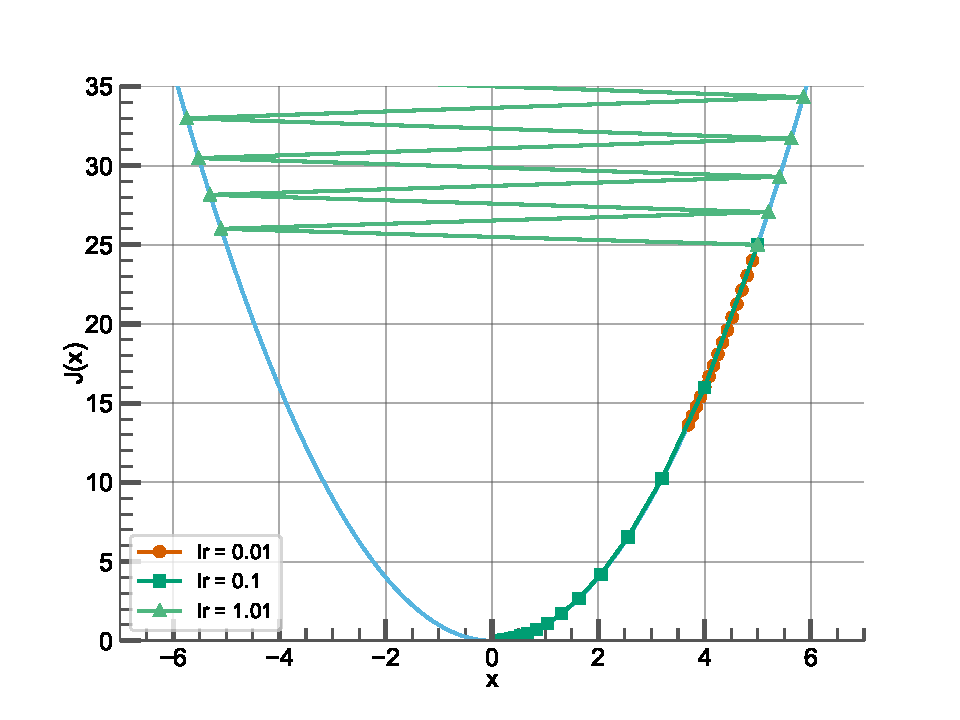
\includegraphics[width=0.7\textwidth]{chapter_dlo/assets/gradient_descent.pdf}
  \caption{Illustration of the effect of the learning rate on the convergence of
    the gradient descent. The gradient descent has been applied iteratively for
    20 epochs. On the one hand, a too-high learning rate ($\eta=1.01$) causes
    the gradient descent to overshoot the minimum of the loss function. On the
    other hand, a too-low learning rate ($\eta=0.01$) causes the gradient
    descent to converge slowly.}
  \label{fig:dlo:gradient_descent}
\end{figure}

\noindent \textbf{Alternative methods.} To enhance the performance of \ac{SGD},
various modifications and extensions have been proposed, such as \ac{SGD} with
momentum \cite{sutskever2013importance,polyak1964some}, RMSProp
\cite{hinton2012neural}, or Adam \cite{kingma2014adam}. These methods aim to
adjust the learning rate dynamically or dampen the oscillations in the gradient
descent to achieve faster and more stable convergence.\\

For instance, \ac{SGD} with momentum
\cite{sutskever2013importance,polyak1964some} uses a momentum coefficient
$\gamma$ and smoothes the variations of the descent direction, thus preventing
the optimisation from getting stuck in small local minima. The momentum term is
a moving average of the gradient, here denoted $v$, and it is used to update the
parameters as shown in \cref{eqn:dlo:sgd_momentum_update}. In this equation, the
momentum coefficient $\gamma \in [0,1]$ is a hyperparameter that is typically
set close to 1, $0.9$ being a common value.\\

\begin{equation}
  \label{eqn:dlo:sgd_momentum_update}
  \begin{split}
    v_{t+1} &= \gamma v_t + \eta \nabla \mathcal{J}(\theta) \\
    \theta_{t+1} &= \theta_t - v_{t+1}
  \end{split}
\end{equation}\\

\section{Convolutional Neural Networks for Computer Vision}\label{sec:dlo:cnn}

In the field of computer vision, \acp{CNN} have emerged as effective
architectures that enable high performance on image classification tasks. The
effectiveness of \acp{CNN} lies in their architecture that leverages the \ac{CL}
layers to automatically learn abstract features from visual data in a
hierarchical fashion. In this section, we explore the building blocks of
\acp{CNN} and various architectures that have been widely used and became
\emph{de facto} standards in the literature.

\subsection{Building Blocks}

This section covers the most common building blocks of \acp{CNN} for computer
vision. These building blocks are organised in layers that are stacked to form
neural network architectures subsequently detailed in
\cref{sec:dlo:architectures,sec:dlo:architectures_used}.\\

\noindent\textbf{Convolutional layer.} \ac{CL} layers are one of the core
building blocks of \acp{CNN}. Each convolution layer performs a series of
spatial convolutions on the input data using a set of learnable filters or
kernels. These filters are designed to extract low-level features such as edges,
corners, and textures in the early layers, while they learn high-level features
like object parts or even whole objects in the deeper layers. Contrary to manual
feature engineering, the features learned by \ac{CL} layers are learned in a
\emph{end-to-end} fashion. The 2D convolution operation is defined in
\cref{eqn:dlo:convolution} :\\

\begin{equation}
  \label{eqn:dlo:convolution}
  % (x * k)(i,j) = \sum_{m} \sum_{n} x(i -m, j -n) \cdot k(m, n)
    Y_{ij} = \sum_{{a=0}}^{{k_h-1}} \sum_{{b=0}}^{{k_w-1}} X_{i-a, j-b} \cdot K_{ab}    
\end{equation}\\

\noindent where $\mathbf{X}$ is the input, $\mathbf{K}$ is the kernel of size
$k_h \times k_w$ and $(i,j)$ are the spatial coordinates in the output feature
map. Note that some Deep Learning frameworks implement \emph{cross-correlation}
instead of convolution. In the former, the kernel is not spatially flipped
leading to the cross-correlation not being commutative
\cite{goodfellow2016deep}. The \ac{CL} layer kernels are typically smaller than
the input along width and height dimensions (they are generally $3\times 3$
\cite{DBLP:conf/cvpr/HeZRS16}) but comprise as much channels as the input.
During the forward pass, each kernel is spatially convolved channel-wise with
the input and the convolution outputs are summed along the channel dimension to
yield a single scalar for each kernel position on the input (see also
\cref{fig:dlo:conv_layer}).\\

\ac{CL} layers are more computationally efficient than \ac{FC} layers, as they
have a form of weight sharing baked in. Indeed, the same kernel is applied to
every location of the input, which brings two main benefits: \emph{(i)} the
number of parameters is independent of the input size and \emph{(ii)} a single
learned kernel, acting as a feature detector, can be used in multiple locations.
This is especially useful for early feature detector that detects basic shapes
or textures. In addition, because of the kernels being convolved across the
whole input, \ac{CL} layers are also less sensitive to spatial translations that
might occur in different instances of the same class.\\

\noindent \textbf{Fully connected layer.} \ac{FC} layers, also known as
\emph{Dense} layers are often the last layers of a \ac{CNN}, effectively serving
as a classifier, whereas the \ac{CL} layers act as a feature extractor.
\ac{FC} layers perform high-level reasoning by conducting non-linear
transformations of the extracted features and combining them to make decisions.
In an FC layer, each neuron is connected to every neuron in the previous layer.
A \ac{FC} layer can be described as a matrix-vector product as in
\cref{eqn:dlo:fc_layer} (see \cref{fig:dlo:dense_layer}).\\

\begin{equation}
  \label{eqn:dlo:fc_layer}
  \mathbf{y} = \mathbf{w}^T \cdot \mathbf{x} + \mathbf{b}
\end{equation}\\

\noindent where $\mathbf{x}$ is the input vector, $\mathbf{w}$ is the weight
matrix and $b$ is the bias. In the context of \acp{CNN}, before passing the
output of the last \ac{CL} layer to the first \ac{FC} layer, it needs to be
flattened or reshaped into a single column vector. The final layer in a \ac{CNN}
is a \ac{FC} layer that has a number of neurons equal to the number of output
classes, and it typically uses a softmax activation to output a probability
distribution over those classes.\\


\begin{figure}[htbp]
  \centering
  \subfloat[Convolutional Layer\label{fig:dlo:conv_layer}]{
    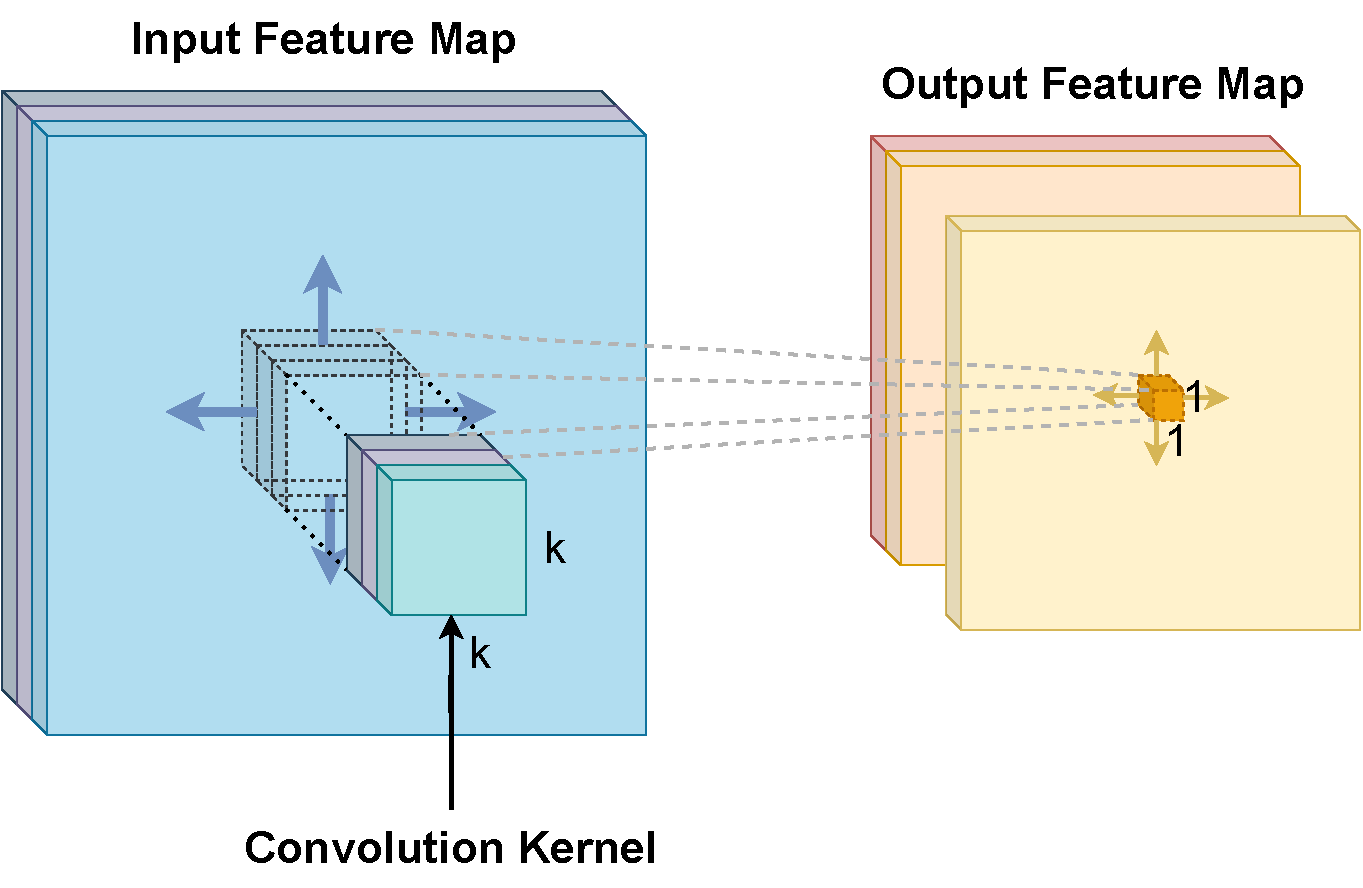
\includegraphics[width=0.49\textwidth]{chapter_dlo/assets/conv_layer.pdf}}
    \subfloat[Fully Connected Layer\label{fig:dlo:dense_layer}]{
    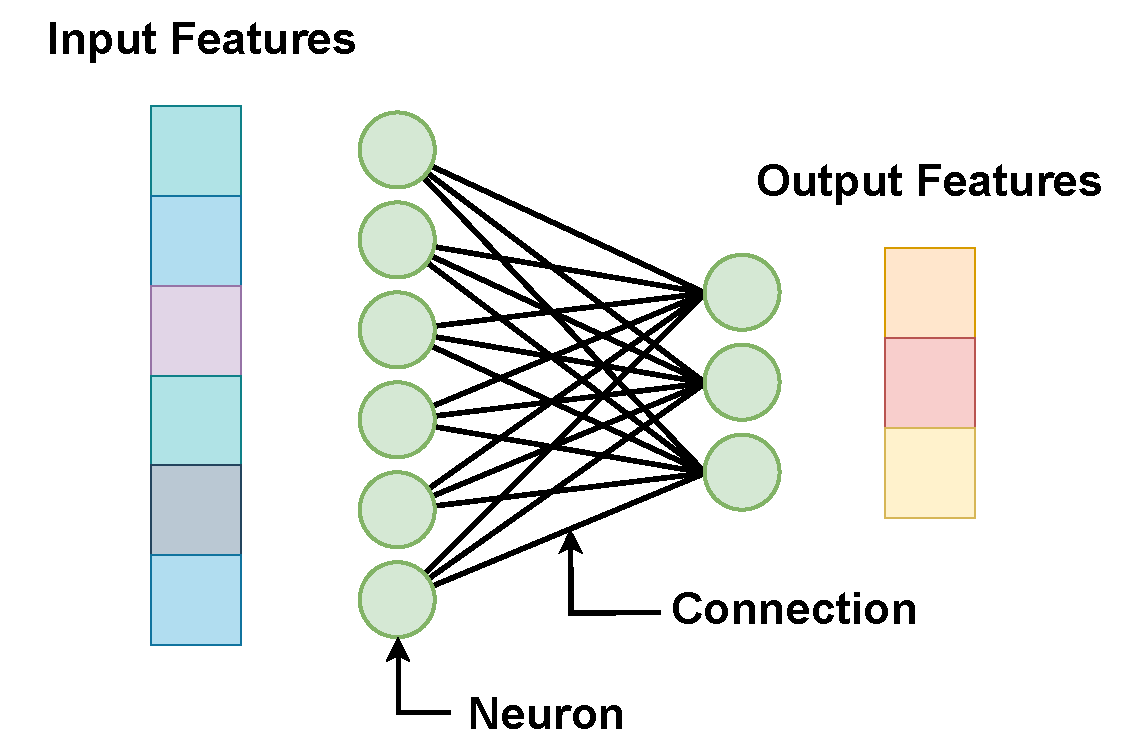
\includegraphics[width=0.49\textwidth]{chapter_dlo/assets/dense_layer.pdf}}
    \caption{Conceptual representation of a \acl{CL} and a \acl{FC} layer. The
    \acl{CL} layer (\cref{fig:dlo:conv_layer}) takes a multi-channel input and
    produces a multi-channel output. Each coefficient of the output is computed
    by applying a convolution operation at a corresponding location in the
    input. The \acl{FC} layer (\cref{fig:dlo:dense_layer}) takes a vector input
    and produces a vector output. Each connection is represented by a weight in
    the weight matrix.}
  \label{fig:sota:layers}
\end{figure}

\noindent \textbf{Activation functions.} They are often applied to the output
feature map of a convolutional or fully connected layer, resulting in the
\emph{activation map} or \emph{activations}. These functions introduce
non-linearity into the model, allowing it to learn more complex patterns
\cite{long2015fully}. A common activation function used in \acp{CNN} is the
\ac{ReLU}, represented as $f(x)=\max(0,x)$. Other functions like the sigmoid
$f(x)=1/(1+e^{-x})$ or tanh $f(x)=(e^{x} -e^{-x})/(e^{x}+e^{-x})$ functions have
been used (see \cref{fig:dlo:activation_functions}), however, the \ac{ReLU} is
preferred over the latter for its computational efficiency and its ability to
mitigate the vanishing or exploding gradient problem
\cite{hochreiter2001gradient,glorot2010understanding}.\\

\begin{figure}[htbp]
  \centering
  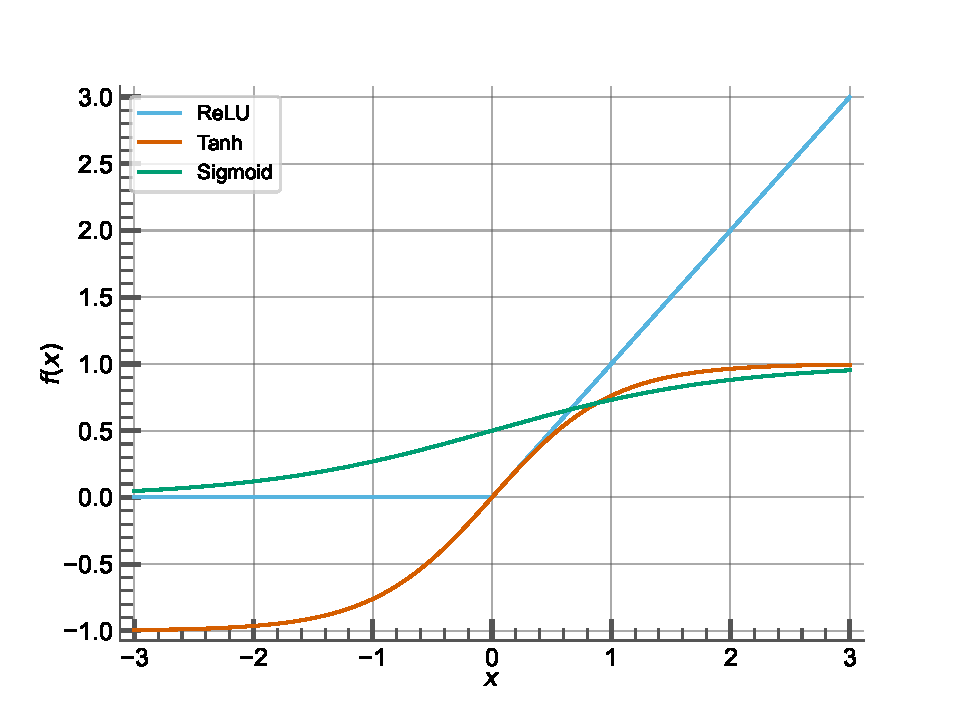
\includegraphics[width=0.7\textwidth]{chapter_dlo/assets/activation_functions.pdf}
  \caption{\ac{ReLU}, tanh and sigmoid activation functions. Best viewed in
  colours.}
  \label{fig:dlo:activation_functions}
\end{figure}

\noindent \textbf{Pooling.} This operation is often employed after \ac{CL}
layers in a \ac{CNN} and aims at progressively reducing the spatial extent of
the input representation, thus reducing the number of parameters and
computations in the network. This also helps control overfitting and increases
the receptive field of the subsequent layers. The pooling operation is performed
independently on each input channel, so the number of channels remains
unchanged. The two most common types of pooling are \emph{max} and \emph{average
pooling}. The former selects the maximum value in each window (often of size
$2\times 2$), while the latter computes the average value of the window. Given
an input matrix $\mathbf{X}$, the output matrix $ \mathbf{Y} $ for a certain
spatial location $(i, j)$ is defined in \cref{eqn:dlo:max_pooling} for \emph{max
pooling} and \cref{eqn:dlo:avg_pooling} for \emph{average pooling}:\\

% \begin{equation}
%   \label{eqn:dlo:pooling}
%   Y_{ij} = p \left( \mathbf{X}(i⋅s:i⋅s+f,j⋅s:j⋅s+f) \right)
% \end{equation}\\

% Max Pooling
\begin{equation}
  \label{eqn:dlo:max_pooling}
  Y^{\text{max}}_{ij} = \max_{(a,b) \in [0, k_h-1] \times [0, k_w-1]} X_{i + a, j + b}
\end{equation}\\
  
  % Average Pooling
  \begin{equation}
  \label{eqn:dlo:avg_pooling}
  Y^{\text{avg}}_{ij} = \frac{1}{k_h \times k_w} \sum_{a=0}^{k_h-1} \sum_{b=0}^{k_w-1} X_{i + a, j + b}  
\end{equation}\\

\noindent where $k_h$ and $k_w$ represent the height and width of the pooling
windows respectively. Note that pooling has no learnable parameters. It only
downsamples the input based on a fixed function.\\


\noindent \textbf{Batch Normalisation.} \ac{BN} is a technique introduced in
\cite{DBLP:conf/icml/IoffeS15} to combat the issue of internal covariate shift
in deep neural networks, thereby accelerating training and improving
generalization. Covariate shift refers to the changes in the distribution of
features in the training and test dataset, which can lead to slow convergence,
make the network harder to train or hinder its generalisation capabilities.
\ac{BN} normalises the input of the layer by adjusting and scaling the
activations of the previous one. For each mini-batch of inputs (for instance,
the activation map of the previous layer), it computes the mean and variance of
the activations and performs normalization. The transformation is defined as
follows:\\

\begin{equation}
  \label{eqn:dlo:batchnorm}
  \hat{x}_{i} = \frac{x_{i} - \mu_{B}}{\sqrt{\sigma_{B}^{2} + \varepsilon}}
\end{equation}\\

\noindent where $x_{i}$ is the input, $\mu_{B}$ is the mini-batch mean,
$\sigma_{B}^{2}$ is the mini-batch variance, and $\varepsilon$ is a small
constant for numerical stability. After normalization, the method allows the
network to learn an affine transformation for each activation, permitting the
network to control the mean and standard deviation of the input distribution,
formalised in \cref{eqn:dlo:batchnorm}:\\

\begin{equation}
  \label{eqn:dlo:batchnorm_affine}
  y_{i} = \gamma \hat{x}_{i} + \beta
\end{equation}\\

\noindent where, $\gamma$ and $\beta$ are the learnable parameters of the affine
transformation. \ac{BN} has the advantage of making the network less sensitive
to the initial weights, allowing higher learning rates, and reducing the need
for Dropout, among other regularisers. However, its effectiveness decreases in
the case of small batch sizes, as the estimate of the batch mean and variance
becomes less accurate.\\

\noindent \textbf{Dropout.} Dropout is a regularization technique used to
prevent overfitting in neural networks. Dropout was introduced in
\cite{DBLP:journals/jmlr/SrivastavaHKSS14} and works by randomly deactivating a
proportion of neurons in a layer during each training iteration. More
specifically, during the forward pass, each neuron has a probability $p$ of
being temporarily removed from the network, effectively breaking up
co-adaptations between neurons and forcing them to learn more robust and
independent features. The output of Dropout is given in \cref{eqn:dlo:dropout}:\\

\begin{equation}
  \label{eqn:dlo:dropout}
    r_i \sim \text{Bernoulli}(1 - p), \quad
    \mathbf{y} = \frac{\mathbf{x} \odot \mathbf{r}}{1 - p} 
\end{equation}\\

\noindent In the above equation, $\mathbf{x}$ denote the output of a layer
processed with dropout, $\mathbf{r}$ is a binary mask vector of the same shape
as $\mathbf{x}$, where each element of $\mathbf{r}$ is independently drawn from a
Bernoulli distribution with probability $1-p$, leading to $r_i=1$ if the
associated weight is kept and a $r_i=0$ if not. The product $\mathbf{x} \odot
\mathbf{r}$ is scaled by $1-p$ to ensure that the expected value of $\mathbf{x}$
remains unchanged. During the evaluation, the dropout is changed to an identity
function.

\subsection{Architectures Evolution}\label{sec:dlo:architectures}

The evolution of \aclp{CNN} is characterised by a consistent increase in their
size and performance, alongside the introduction of new architectural
modifications to address the limitations of their predecessors (see
\cref{fig:dlo:net_sizes}). In this section, we present a historical overview of
the \acp{CNN} evolution and we subsequently detail the architectures that we
used in our experiments.\\

One of the earliest \ac{CNN} was introduced in 1998: LeNet-5 was developed for
digit recognition \cite{DBLP:journals/pieee/LeCunBBH98}, constituting a
relatively simple network with 5 layers with learnable parameters: 2 \ac{CL}
layers and 3 fully connected layers. Its size is significantly smaller compared
to the contemporary models (see \cref{fig:dlo:net_sizes}). With the introduction
of AlexNet \cite{DBLP:conf/nips/KrizhevskySH12} in 2012, the network size
considerably grew, comprising more layers and neurons to handle more complex
tasks, like large-scale image recognition. AlexNet tackled the overfitting
issue in LeNet-5 using data augmentation and dropout techniques, while also
introducing and popularising the \ac{ReLU} activation function.\\

\begin{figure}[htbp]
  \centering
  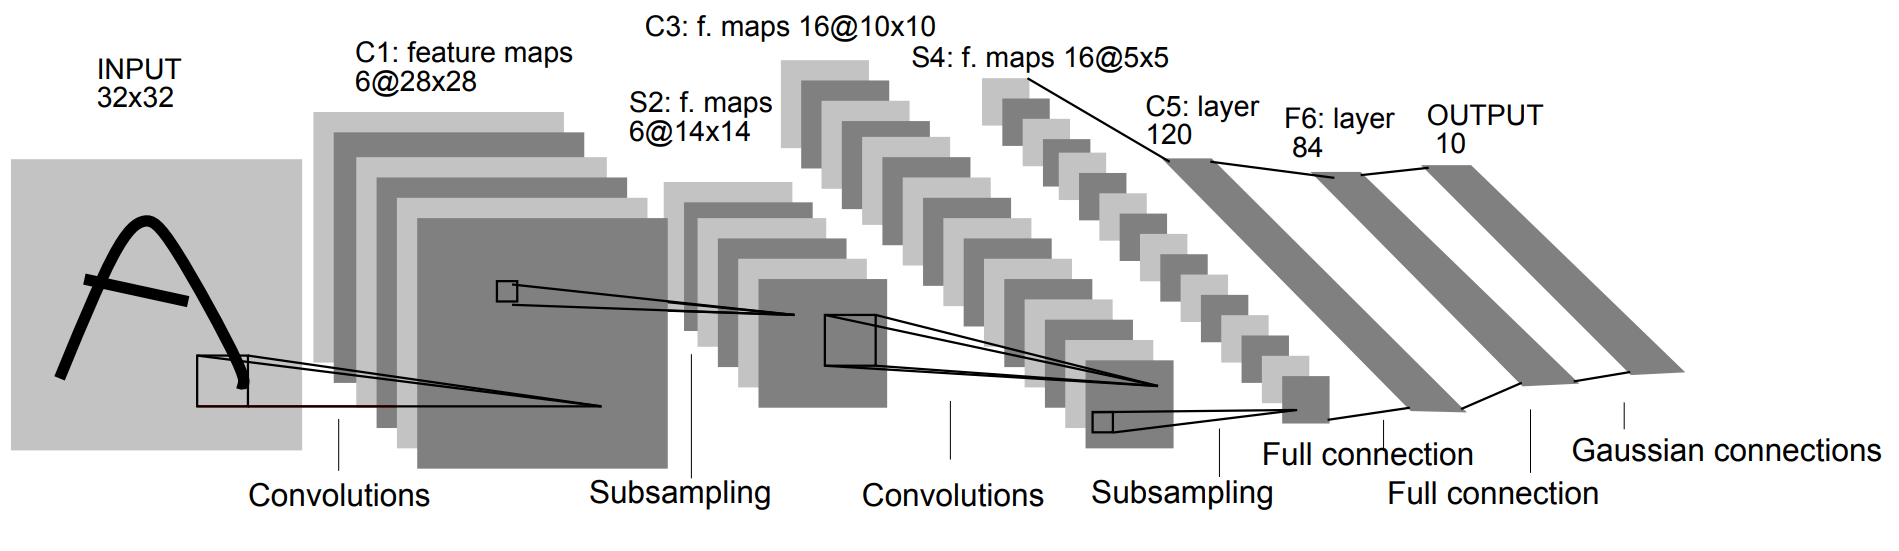
\includegraphics[width=0.70\textwidth]{chapter_sota/assets/lenet.png}
  \caption{Architecture of LeNet-5, a \acl{CNN} used for handwritten digit
    recognition. Image taken from \cite{DBLP:journals/pieee/LeCunBBH98}}
  \label{fig:dlo:lenet5}
\end{figure}


The next advancement was the VGG networks family
\cite{DBLP:journals/corr/SimonyanZ14a} %, introduced in 2014 
which proposed much deeper architectures with up to 19 layers, which is a
significant increase over the 8 layers of AlexNet. However, the increased depth
led to the \emph{vanishing gradient} problems, which refers to the situation in
training a deep neural network where gradients are backpropagated through layers
and become increasingly small, effectively preventing the weights of earlier
layers from learning and updating effectively. The VGG networks also introduced
the practice of stacking multiple convolutional layers with small $3\times 3$
filters instead of using larger ones. The same year, Google's Inception (or
GoogLeNet) \cite{DBLP:conf/cvpr/SzegedyLJSRAEVR15} was introduced, addressing
the vanishing gradient issue with its novel inception modules, which allowed
the network to learn at varying scales and increased computational efficiency,
without overly increasing the network size. GoogleNet was also the first
\ac{CNN} that was not a simple stack of layers and processed a single input with
different blocks in parallel before merging them.\\

\begin{figure}[htbp]
  \centering
  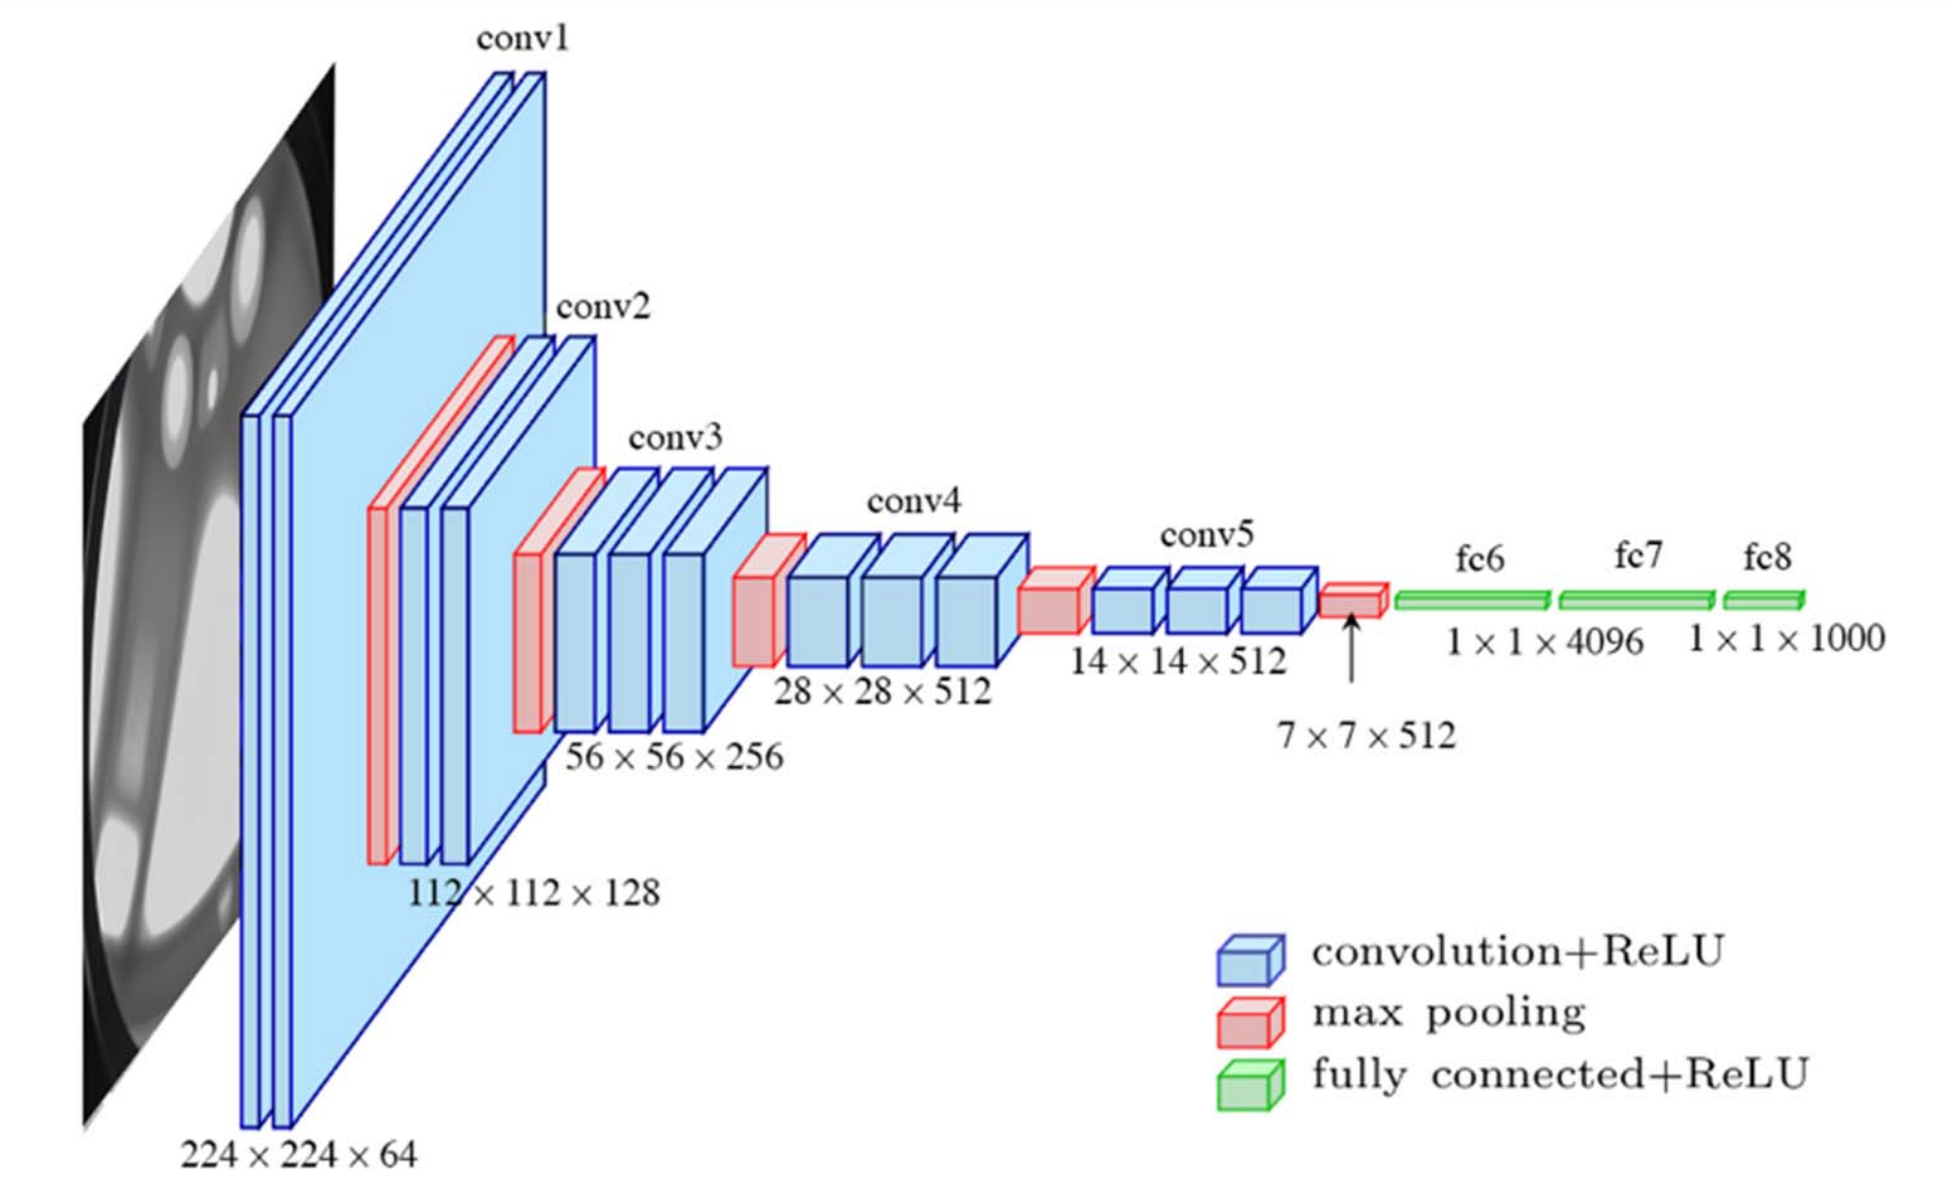
\includegraphics[width=0.7\textwidth]{chapter_sota/assets/vgg16.png}
  \caption{Architecture of the VGG16 network introduced in
    \cite{DBLP:journals/corr/SimonyanZ14a}. Image taken from
    \cite{ferguson2017automatic}}
  \label{fig:dlo:vgg16}
\end{figure}

Later, the ResNet models family was proposed in \cite{DBLP:conf/cvpr/HeZRS16},
which effectively tackled the vanishing gradient problem by introducing skip (or
shortcut) connections, allowing gradients to backpropagate directly through
several layers. These shortcut connections also allowed the network to grow in
depth up to 152 layers without a significant increase in computational cost.
However, a challenge remained with the constant need for careful design to
manage feature-map sizes. Indeed, stacking numerous layers, with their channel
count increasing with depth, can lead to an explosion in the number of
parameters as well as increased memory consumption.\\

\begin{figure}[htbp]
  \centering
  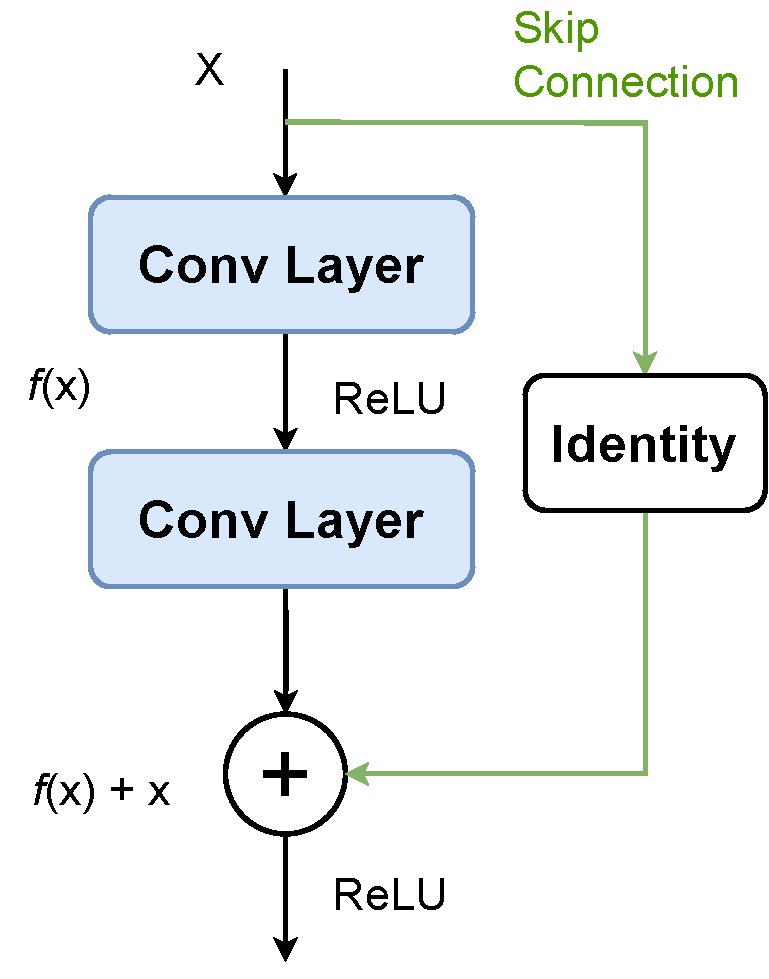
\includegraphics[width=0.5\textwidth]{chapter_dlo/assets/skip_connection.pdf}
  \caption{A residual block and its skip connection used in
    ResNets\cite{DBLP:conf/cvpr/HeZRS16}. The identity skip connection allows
    for the gradient to be backpropagated directly through several layers, thus
    mitigating the \emph{vanishing gradient} problem.}
  \label{fig:dlo:skip_connection}
\end{figure}

In response, DenseNet \cite{huang2017densely} was proposed. It connects each
layer to every other following layer of the same block in a feed-forward
fashion. By reinforcing the propagation of features and gradients through the
network, the DenseNet architecture alleviates the vanishing-gradient problem and
further improves the information flow from earlier layers to later ones by
reusing earlier features in the deeper layers. Thus, through these chronological
advancements, neural networks not only grew in size but also improved in
performance, thereby becoming more efficient and capable of handling more
complex tasks.\\

\begin{figure}[htbp]
  \centering
  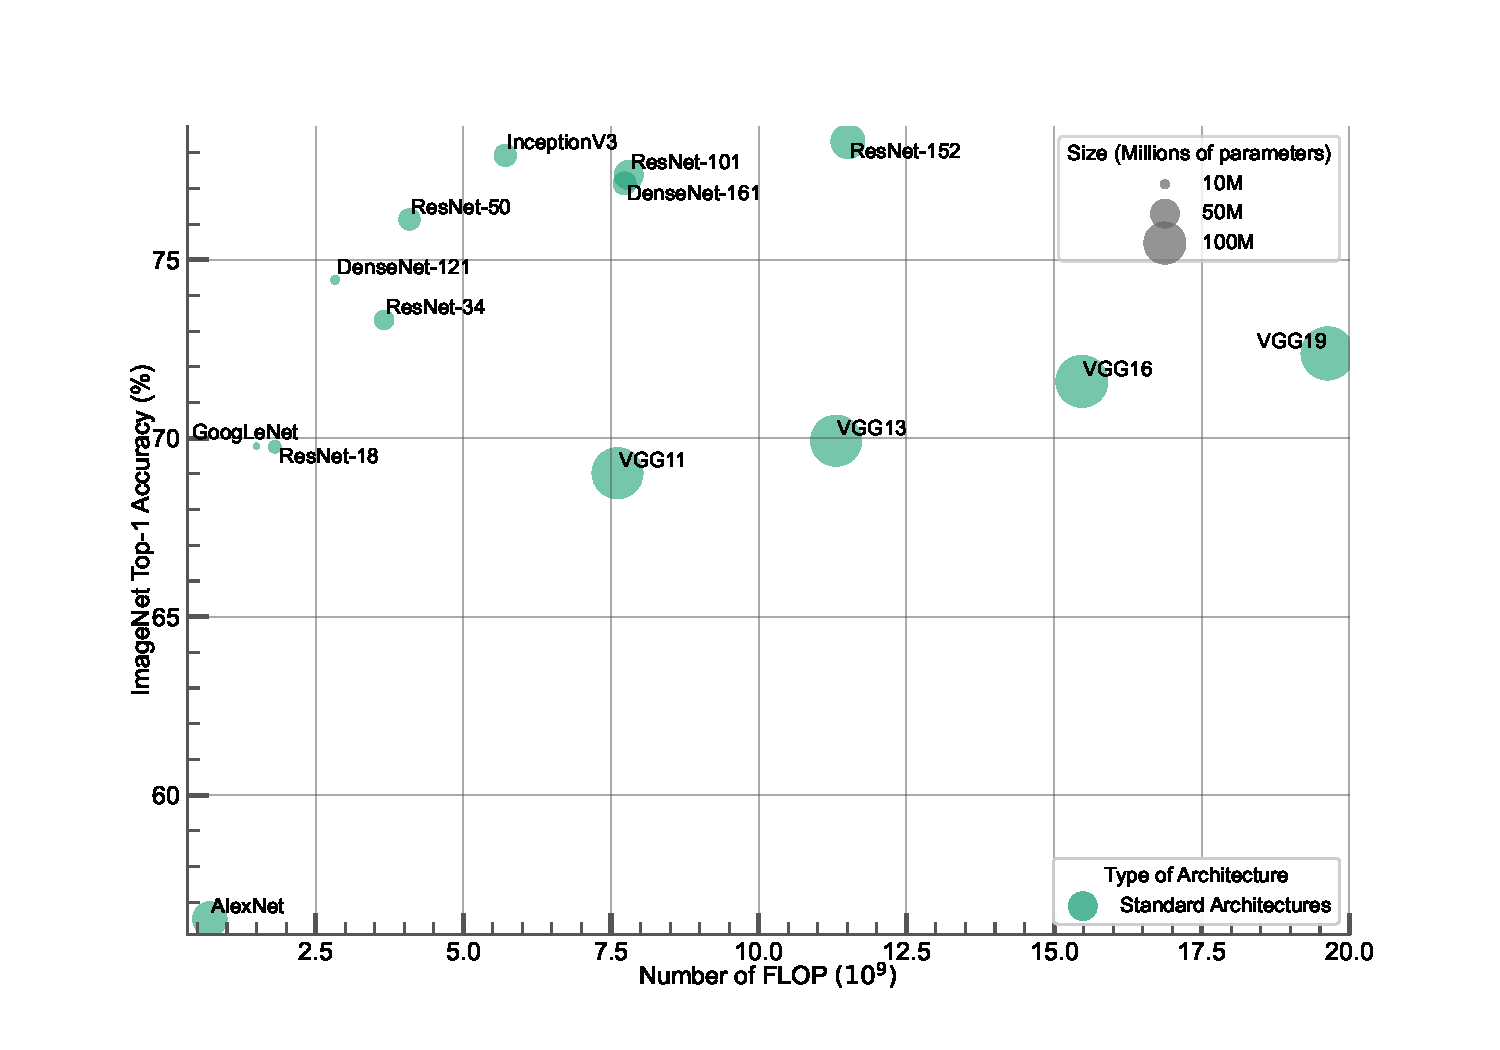
\includegraphics[width=0.7\textwidth]{chapter_sota/assets/network_sizes_normal.pdf}
  \caption{Networks size comparison. The \emph{x-axis} represents the number of
    \acp{FLOP} required to process a single image. The \emph{y-axis} represents
    the Top-1 accuracy on the ImageNet \cite{deng2009imagenet} dataset and the
    size of the circles represents the number of parameters in the network.
    Numbers are taken from \cite{pytorch_vision}}
  \label{fig:dlo:net_sizes}
\end{figure}

\subsection{Architectures Used in Experiments}\label{sec:dlo:architectures_used}

In the subsequent paragraphs, we detail the architectures that we used in our
experiments. We chose these architectures because they are representative of the
state-of-the-art in image classification and they are widely used in the pruning
literature. \Cref{tab:dlo:networks_size} gives an overview of the different
network architectures.\\

\begin{table}[ht!]
  \centering
  \begin{tabular}{lcccccc}
    \cline{2-7}
    & \textbf{Conv2} & \textbf{Conv4} & \textbf{Conv6} & \textbf{VGG16} & \textbf{ResNet20} & \textbf{ResNet18} \\ \hline
    Number of Parameters & 4,301,642 & 2,425,930  & 2,262,602      & 14,728,266
    & 269,034           & 11,685,608 \\
    Number of layers & 5 & 7 & 9 & 14 & 20 & 18 \\
    Number of \ac{CL} layers & 2 & 4 & 6 & 13 & 19 & 17 \\
    Number of \ac{FC} layers & 3 & 3 & 3 & 1 & 1 & 1 \\ \hline
  \end{tabular}
  \caption{Number of parameters for the used neural network architectures. The
  number of parameters is given for the CIFAR-10 dataset, except for the
  ResNet18 architecture, whose number of parameters is given for the
  TinyImageNet dataset.}
  \label{tab:dlo:networks_size}
\end{table}

% VGG16
\noindent \textbf{VGG16.} The VGG16 network
\cite{DBLP:journals/corr/SimonyanZ14a} is a 16-layer \ac{CNN} composed of 13
\ac{CL} layers and 3 fully connected layers. VGG16 was originally designed
for ImageNet \cite{deng2009imagenet} and in our experiments with CIFAR-10 and
CIFAR-100 (described in \cref{sec:dlo:datasets}) we use a slightly modified
version of VGG16 where we replace the 3 \ac{FC} layers with an average pooling
layer and a single \ac{FC} layer \cite{vggcifar}. The \ac{CL} layers
filters are of size $3\times 3$ with a stride of 1. The max-pooling layers are
of size $2\times 2$ with a stride of 2. Each \ac{CL} layer is followed by
a \ac{ReLU} activation function. The VGG16 network is illustrated in
\cref{fig:dlo:vgg16_cifar}.\\

\begin{figure}[htbp]
  \centering
  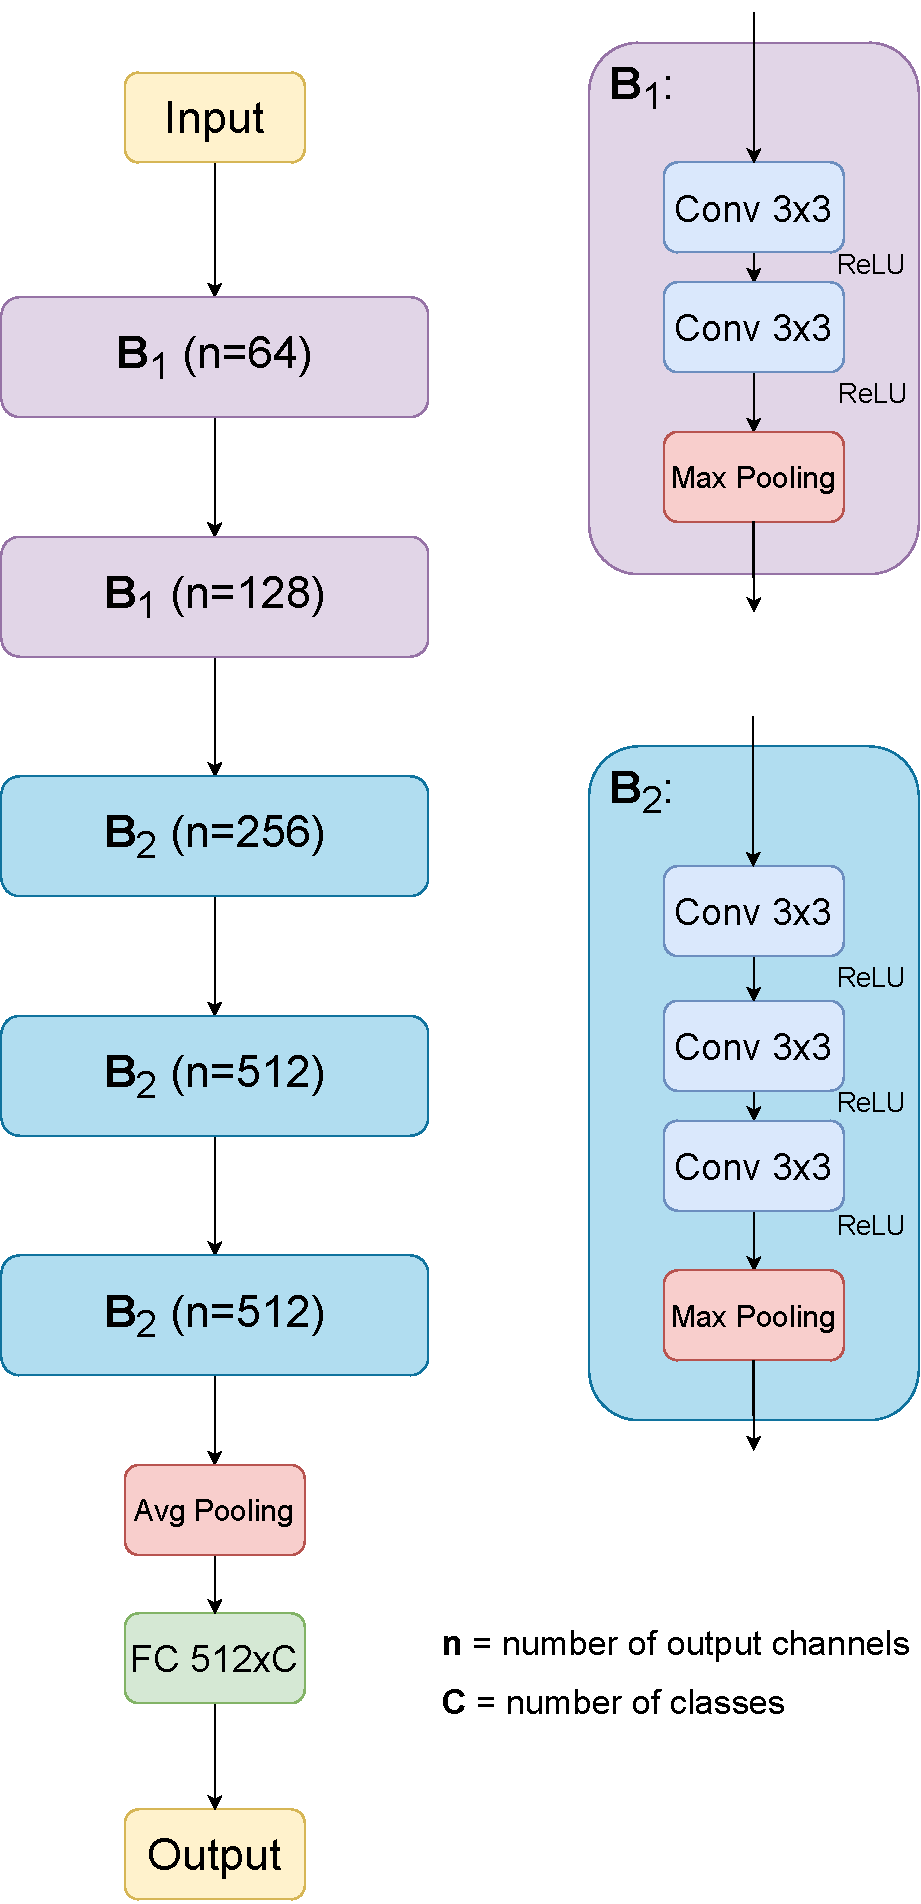
\includegraphics[width=0.30\textwidth]{chapter_dlo/assets/vgg16_cifar.pdf}
  \caption{VGG16 adapted for CIFAR-10 and CIFAR-100.}
  \label{fig:dlo:vgg16_cifar}
\end{figure}

% ResNet18 and ResNet20
\noindent \textbf{ResNet\{18,20\}.} The ResNet18 and ResNet20 networks
\cite{DBLP:conf/cvpr/HeZRS16} are 18 and 20-layer \acp{CNN} respectively. These
layers are organized into stages, with ResNet18, represented in
\cref{fig:dlo:resnet18}, consisting of 4 stages with 2 \emph{Basic Blocks}
(detailed subsequently), while ResNet20, represented in \cref{fig:dlo:resnet20},
is structured into 3 stages, each containing 3 \emph{Basic Blocks}. The
\emph{Basic Blocks}, also referred to as \emph{Residual Blocks}, are composed of
\ac{CL} layers (see \cref{fig:dlo:resnet18,fig:dlo:resnet20}) and follow the
principle of learning the residual function:\\

\begin{equation}
  f(x) = h(x) - x
\end{equation} \\

\noindent where $h(x)$ is the mapping usually learned by previous architectures
such as VGG16. The representation of a residual block is given by
\cref{eqn:dlo:residual_block} (see also \cref{fig:dlo:skip_connection}): \\

\begin{equation}
  \label{eqn:dlo:residual_block}
  y = f(x,\theta) + x
\end{equation}\\

\noindent where $x$ is the input, $f$ represents the residual function, $\theta$
are the weights of the block, and $y$ is the output. In
\cref{eqn:dlo:residual_block} $+ x$ denotes the skip connection, which enables
direct backpropagation of the gradient to earlier layers.\\

\begin{figure}
\centering
\subfloat[ResNet20\label{fig:dlo:resnet20}]{
  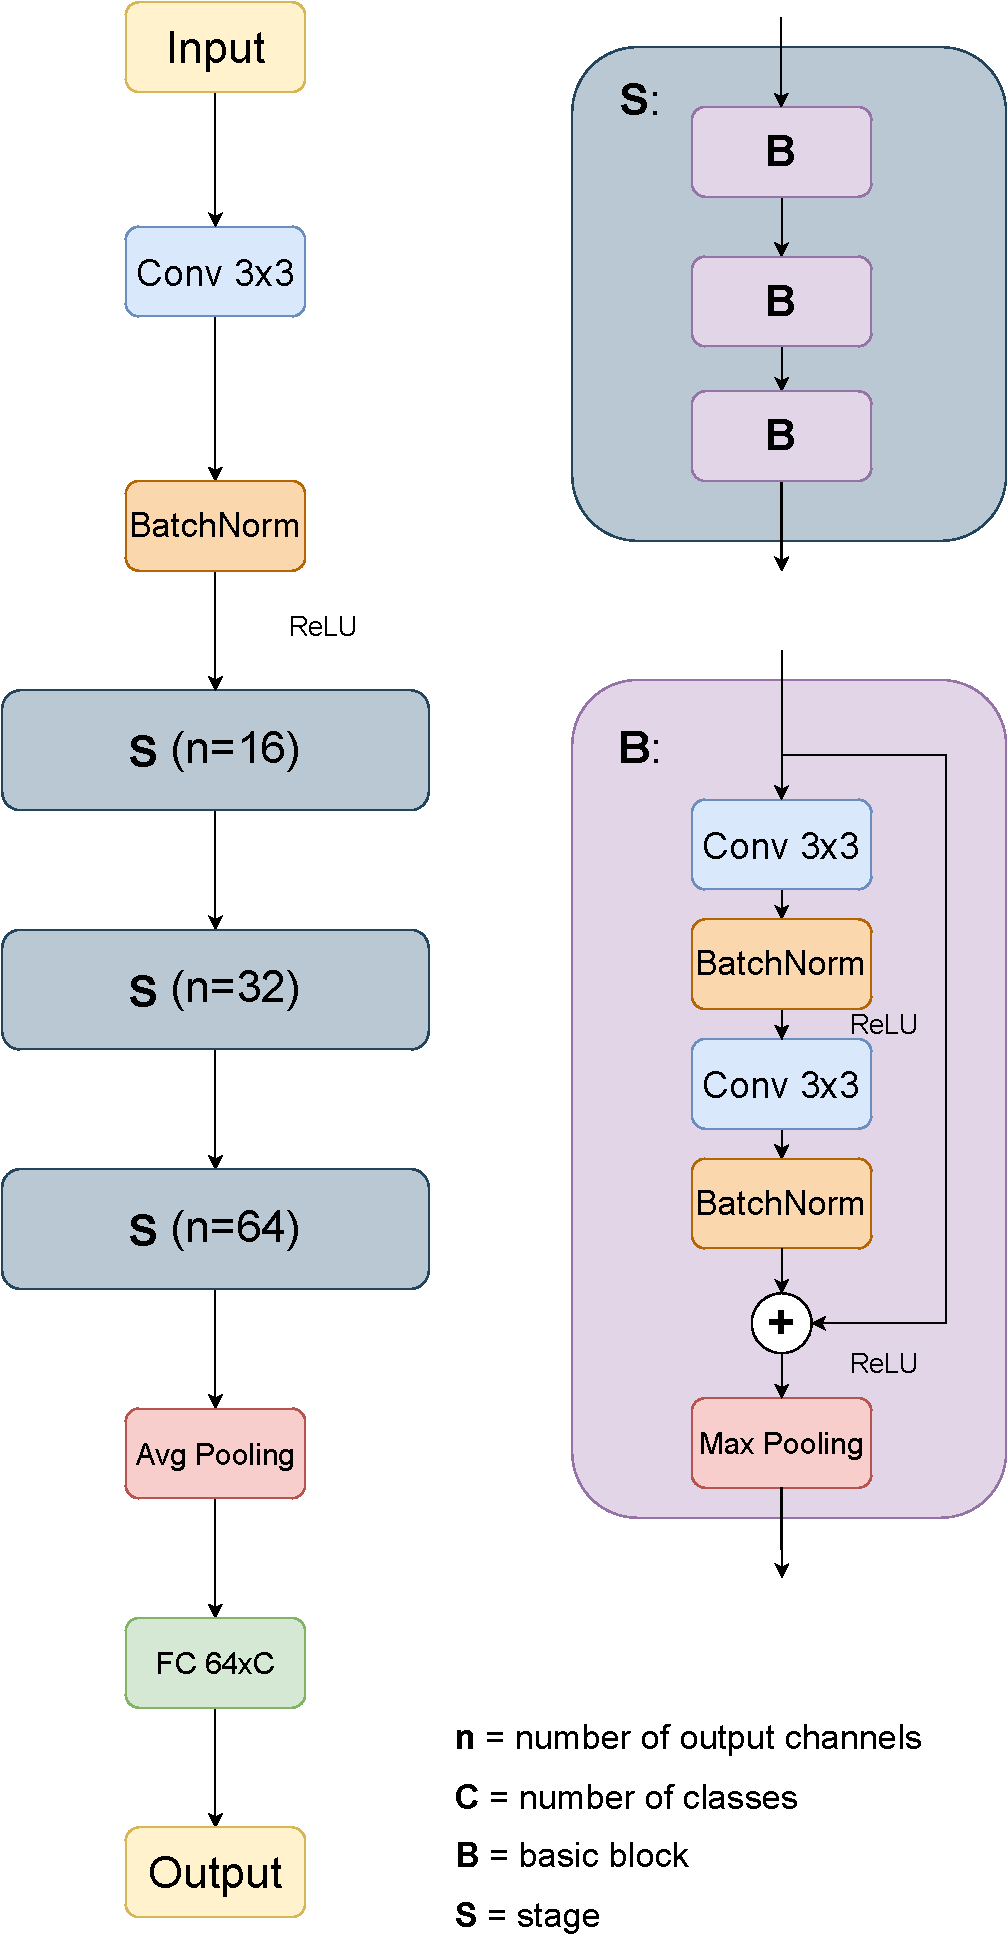
\includegraphics[width=0.35\textwidth]{chapter_dlo/assets/resnet20.pdf}}
  \hfill
\subfloat[ResNet18\label{fig:dlo:resnet18}]{
  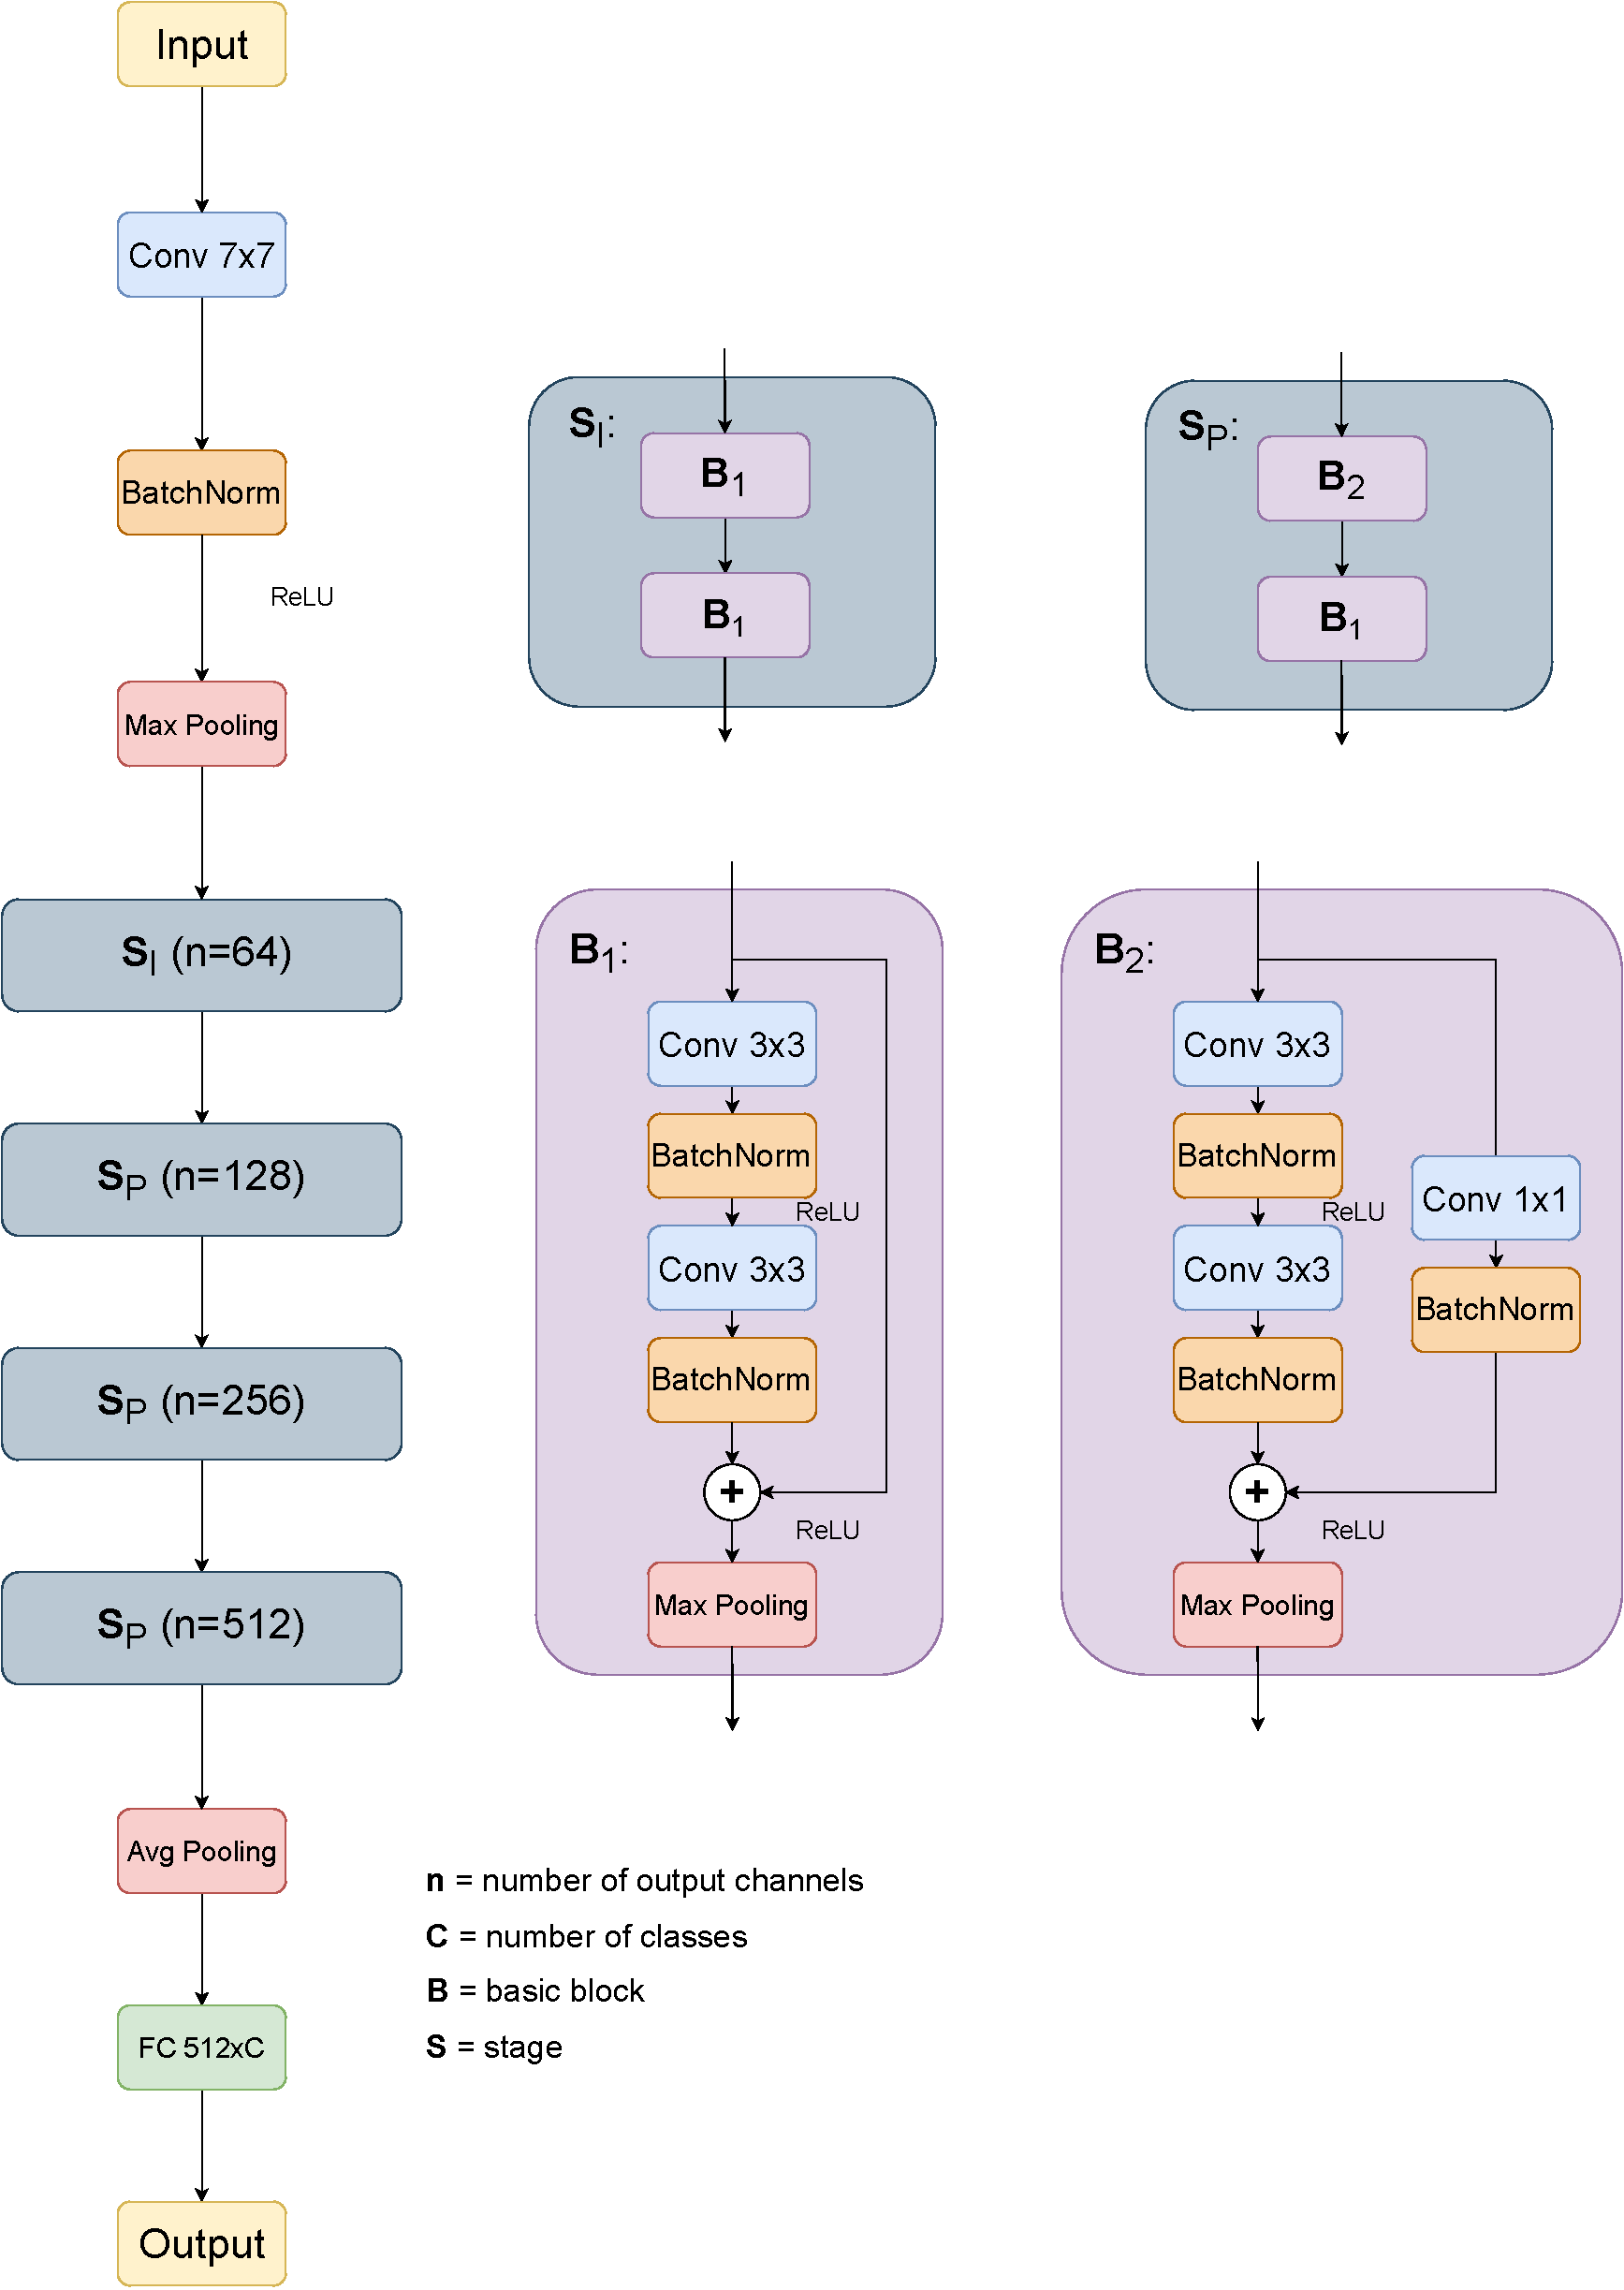
\includegraphics[width=0.60\textwidth]{chapter_dlo/assets/resnet18.pdf}}

\caption{ResNet20 and ResNet18 architectures. ResNet20 (\cref{fig:dlo:resnet20})
is tailored for CIFAR-10 and comprises 3 stages encompassing 3 \emph{Basic
Blocks} of 2 \ac{CL} layers each, with an identity skip connection in each
block. ResNet18 (\cref{fig:dlo:resnet18}) is tailored for ImageNet and is
composed of 4 stages encompassing 4 \emph{Basic Blocks} of 2 convolutional
layers each. There are two types of blocks: $\mathbf{B}_\text{I}$ with an
identity skip connection and $\mathbf{B}_\text{P}$ with a projection skip
connection. The projection skip connection is used to match the dimensions
between the input and the output of the block.}
\label{fig:dlo:resnets}
\end{figure}

\noindent \textbf{Conv\{2,4,6\}.} Conv2, Conv4 and Conv6 are shrunk down
versions of the VGG16 network architecture, composed of 2, 4 and 6 \ac{CL}
layers respectively and 3 \ac{FC} layers. Although Conv2, Conv4 and Conv6,
introduced by \citeauthor{DBLP:conf/iclr/FrankleC19} in
\cite{DBLP:conf/iclr/FrankleC19}, are not widely featured in existing
literature, we chose to employ them due to their use in the methods we benchmark
against. The \ac{CL} layers are stacked in increasing depth, and their
convolutional filters are of size $3\times 3$ with a stride of 1. The
max-pooling layers are of size $2\times 2$ with a stride of 2. They are
represented in \cref{fig:dlo:conv246}.\\

\begin{figure}[htbp]
  \centering
  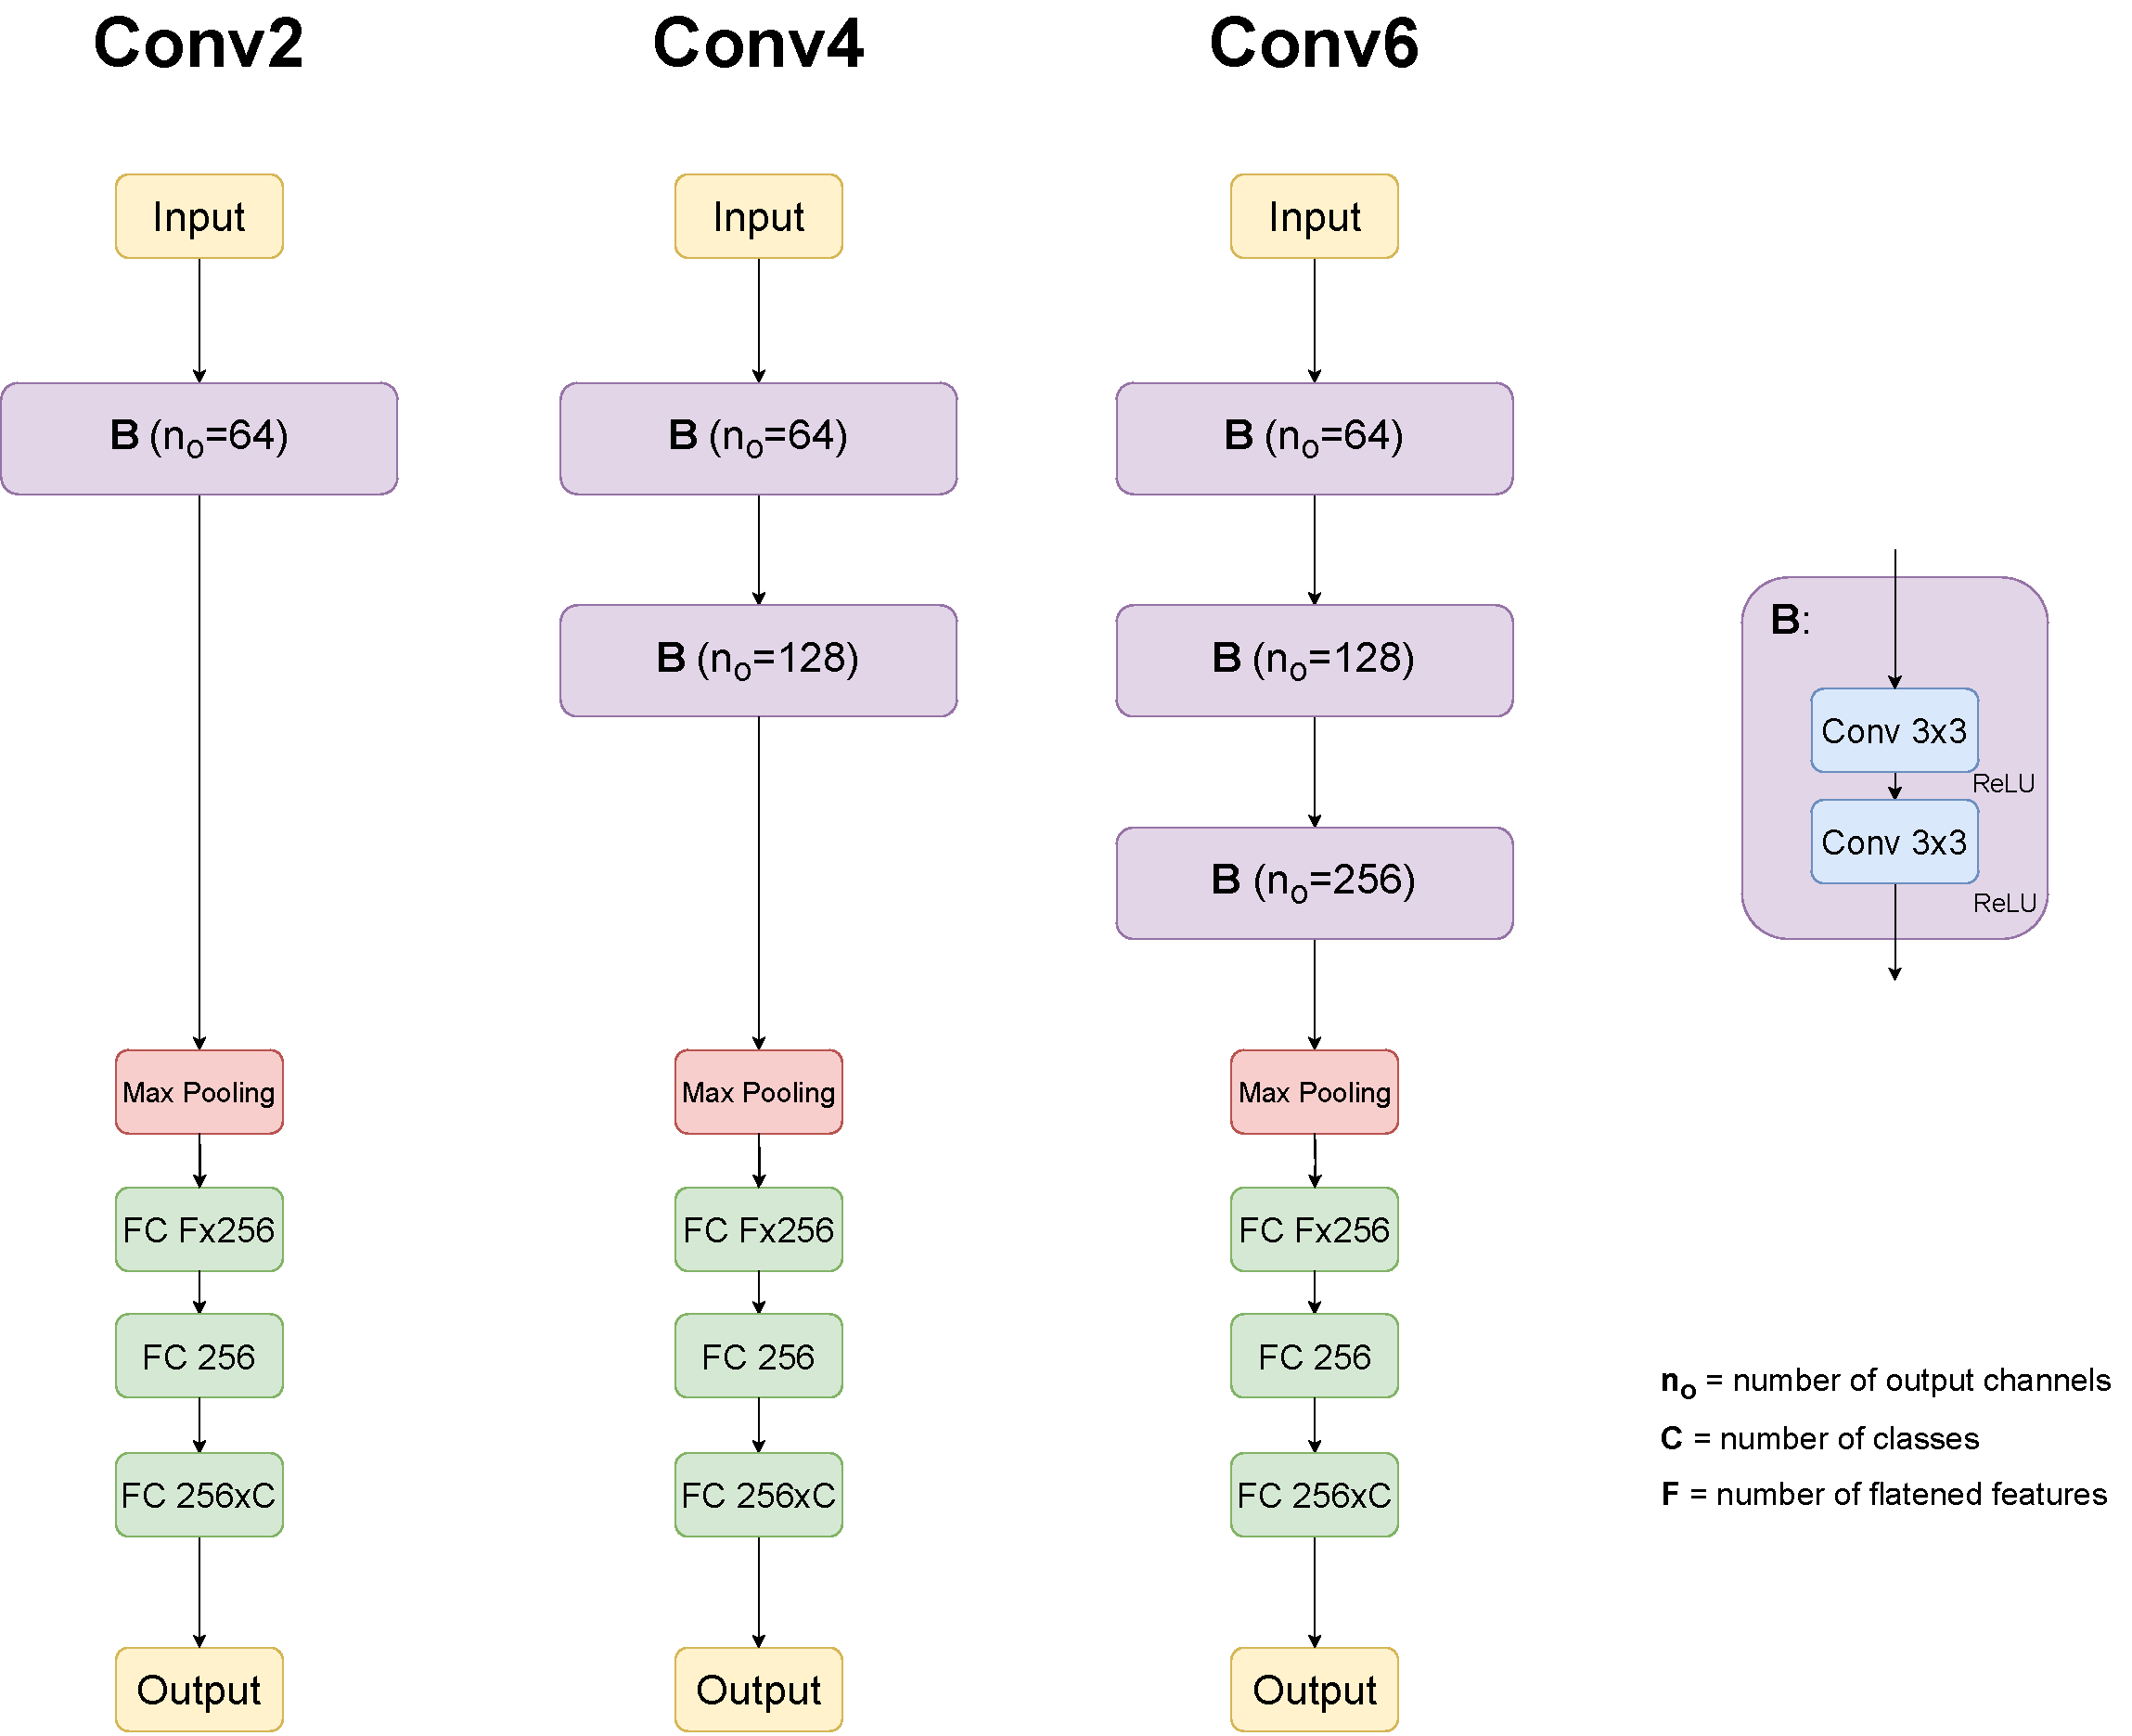
\includegraphics[width=0.7\textwidth]{chapter_dlo/assets/conv246.pdf}
  \caption{Conv2, Conv4 and Conv6 architectures. The number of flat features
  $\mathbf{F}$ corresponds to the size of the feature map of the last block
  $\mathbf{B}$, once vectorised. $\mathbf{F}=16384, ~8192~ \text{and}~ 4096$ for Conv2, Conv4
  and Conv6, respectively for input images of size $32\times 32$.}
  \label{fig:dlo:conv246}
\end{figure}


\section{Datasets}\label{sec:dlo:datasets}

In this thesis, we focus on image classification and supervised learning, a
machine learning paradigm in which the model is trained using labelled data. In
the context of image classification, the labelled data are pairs of images and
labels which represent the class of their associated image. We denote an input
image $X$ and its corresponding label $y$. Each image $X$ belongs to the set of
all images of the dataset $\mathcal{X}$, and each label $y$ belongs to the set
of all labels of the dataset $\mathcal{Y}$. The ensemble of the image-label
pairs are gathered in a dataset, denoted $\mathcal{D}$, which is formally a set
of pairs $(X, y)$, where $X \in \mathcal{X}$ and $y \in \mathcal{Y}$, so that
$\mathcal{D} \subset \mathcal{X} \times \mathcal{Y}$. \\

Following these formal notations, the subsequent sections give details about the
datasets used in our experiments. We evaluated our methods on three different
datasets tailored for image classification: CIFAR-10 \cite{CIFARdataset},
CIFAR-100 \cite{CIFARdataset} and TinyImageNet \cite{TinyImageNet}. The
following paragraphs give details about these datasets and
\cref{tab:dlo:datasets} sums up their main characteristics.\\

\begin{table}[ht!]
  \centering
  \begin{tabular}{lcccc}
    \toprule
    \textbf{Dataset}    & \textbf{Number of images} & \textbf{Number of classes} &
    \textbf{Image size} & \textbf{Size of test set}                                               \\
    \hline
    CIFAR-10            & 60,000                    & 10                         & 32x32 & 10,000 \\
    CIFAR-100           & 60,000                    & 100                        & 32x32 & 10,000 \\
    TinyImageNet        & 100,000                   & 200                        & 64x64 & 10,000 \\
    \bottomrule
  \end{tabular}
  \caption{The number of images, of classes, image size and size of the test
    set for the three datasets used: CIFAR-10, CIFAR-100 and TinyImageNet.}
  \label{tab:dlo:datasets}
\end{table}

\subsection{CIFAR-10}

CIFAR-10 \cite{CIFARdataset} is a widely used dataset in machine learning and
computer vision. This is a labelled subset of the \emph{80 Million Tiny Images}
dataset \cite{4531741}. CIFAR-10 is a simple yet challenging dataset that allows
for quicker iteration or hyperparameter tuning than larger datasets such as
ImageNet \cite{DBLP:journals/ijcv/RussakovskyDSKS15}, but it is significantly
more complex than the MNIST dataset \cite{6296535}, which contains grayscale
handwritten digits images. The CIFAR-10 dataset contains 60,000 colour images of
size 32x32 pixels, split into 10 classes, namely: plane, car, bird, cat, deer,
dog, horse, ship, and truck. Each class contains 6,000 images. The dataset is
divided into two subsets: a training set, composed of 50,000 images and a test set
containing 10,000 of them.\\

\begin{figure}[ht!]
  \centering
  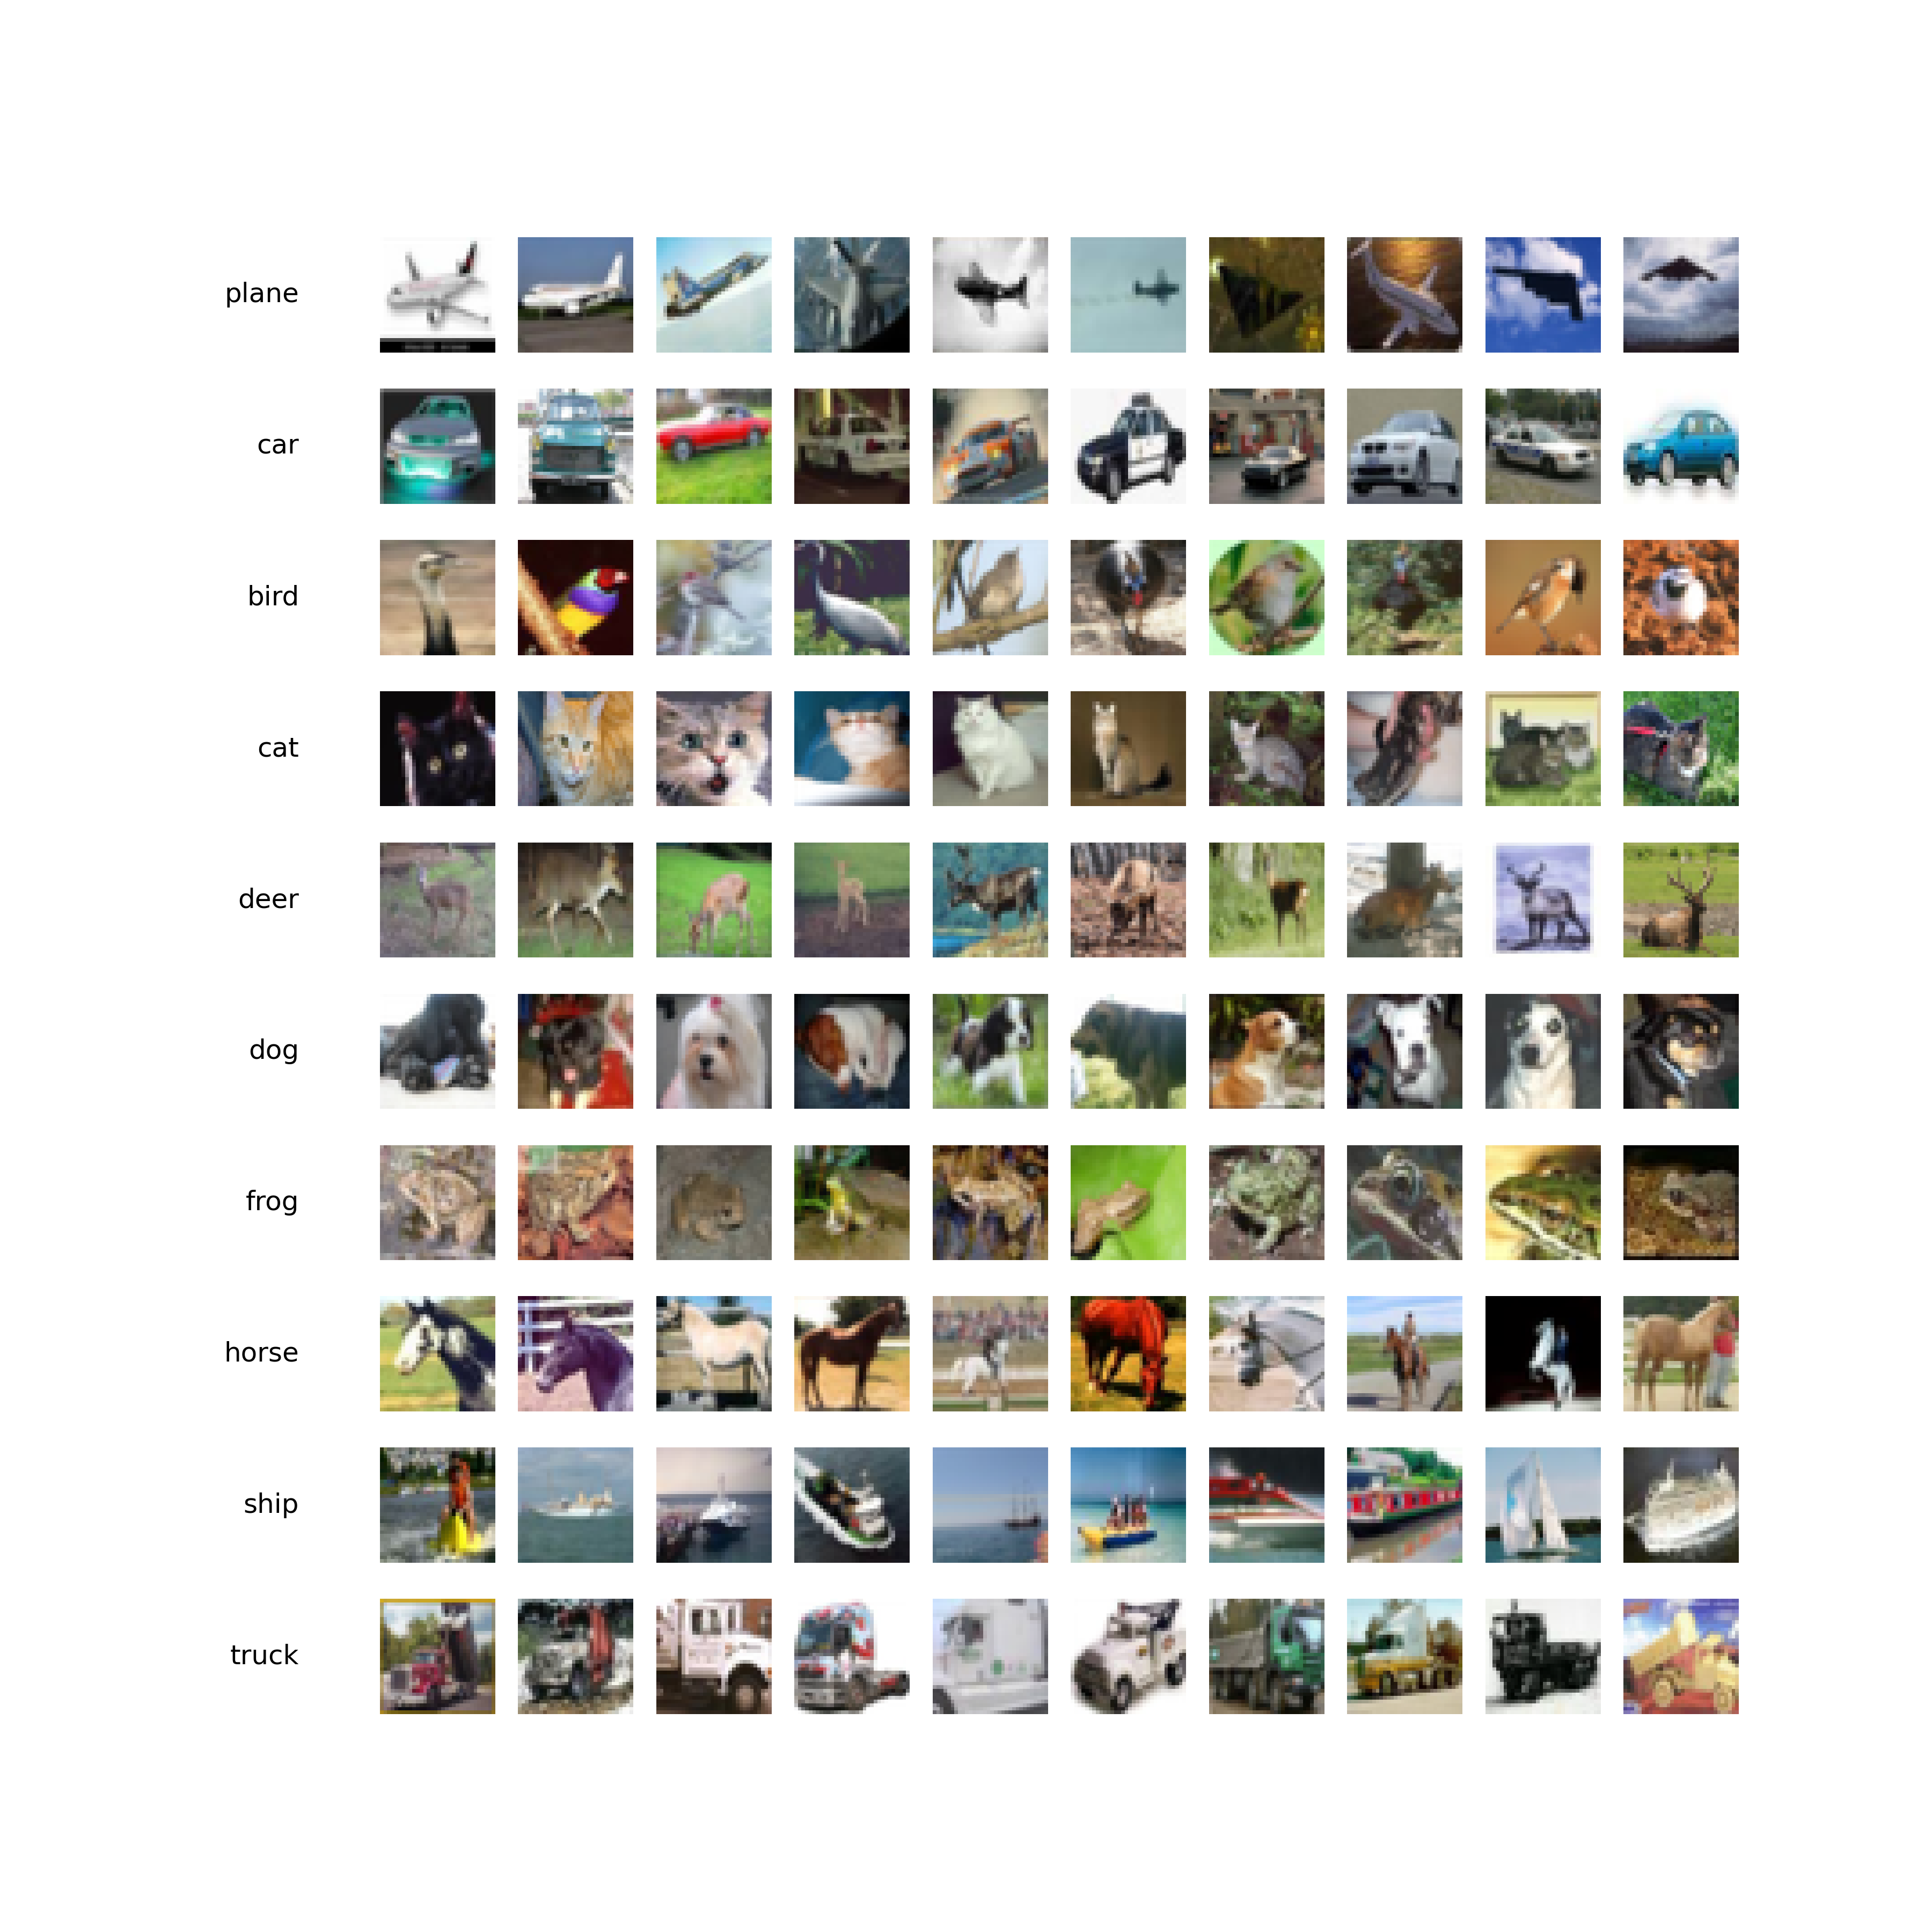
\includegraphics[width=0.7\textwidth]{chapter_dlo/assets/cifar-10_example.png}
  \caption{ A sample of images from CIFAR-10. Each row contains images from one
    of the 10 classes: plane, car, bird, cat, deer, dog, frog, horse, ship, and
    truck}
  \label{fig:intro:cifar10_examples}
\end{figure}


\subsection{CIFAR-100}

CIFAR-100 \cite{CIFARdataset} is a more challenging
version of CIFAR-10. Like the latter, it is a labelled subset of the \emph{80
  Millions Tiny Images} and  is composed of 60,000 colour images of size 32x32
pixels. However, instead of 10 classes, CIFAR-100 contains 100 classes of 600
images each. As a result, each class has far fewer images than in CIFAR-10.
CIFAR-100 is also divided into two sets: a training and a test set, composed of
50,000 and 10,000 images respectively.\\

\begin{figure}[htbp]
  \centering
  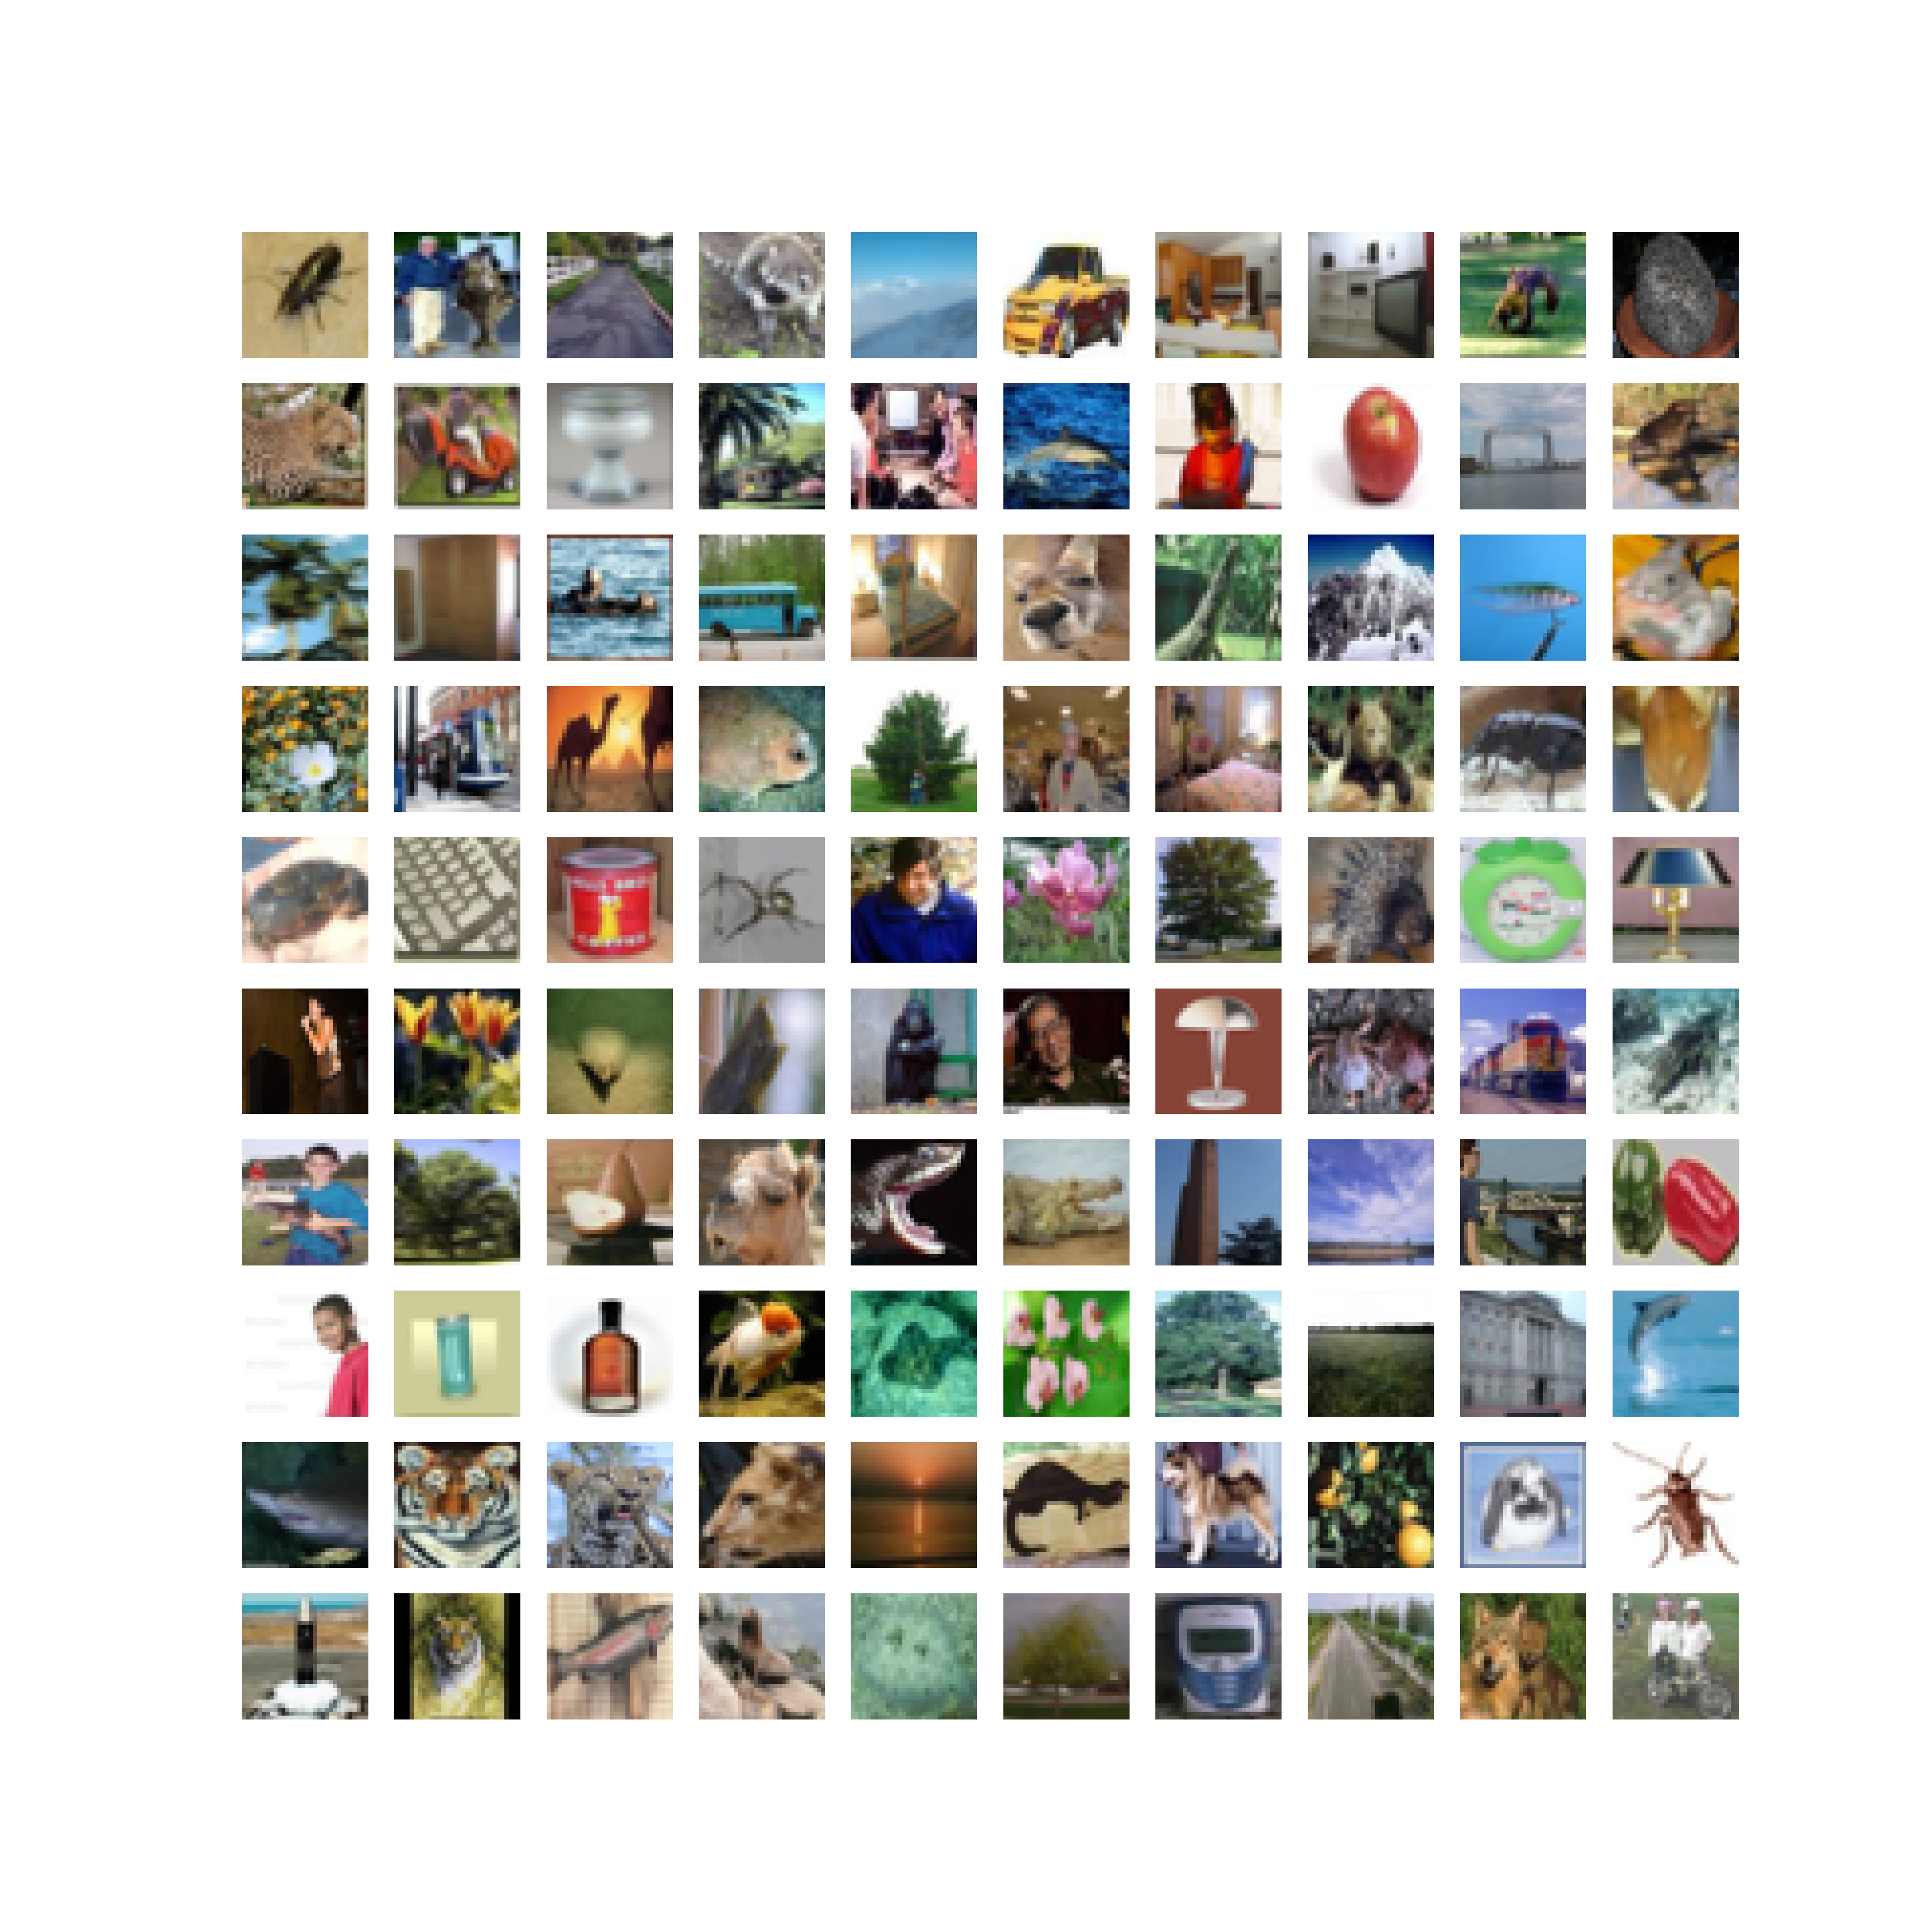
\includegraphics[width=0.7\textwidth]{chapter_dlo/assets/cifar-100_example.png}
  \caption{A sample of images from CIFAR-100. Each image represents an instance
    of one of the 100 distinct classes.}
  \label{fig:intro:cifar100_examples}
\end{figure}


\subsection{TinyImageNet}

TinyImageNet is another popular dataset in machine learning and computer vision,
conceived as a subset of the larger ImageNet dataset
\cite{DBLP:journals/ijcv/RussakovskyDSKS15}. It comprises 100,000 colour images
of size 64x64 pixels, split into 200 classes, whereas ImageNet contains 1.2
million images of size 256x256 pixels, split into 1,000 classes. The dataset is
divided in 3 sets: the train set, which contains 500 images per class, the
validation and test sets, which both contain 50 images. The scaled-down image
size and the reduced number of images make TinyImageNet more computationally
manageable than ImageNet while still being challenging by offering diversity in
the image classes.\\


\begin{figure}[htbp]
  \centering
  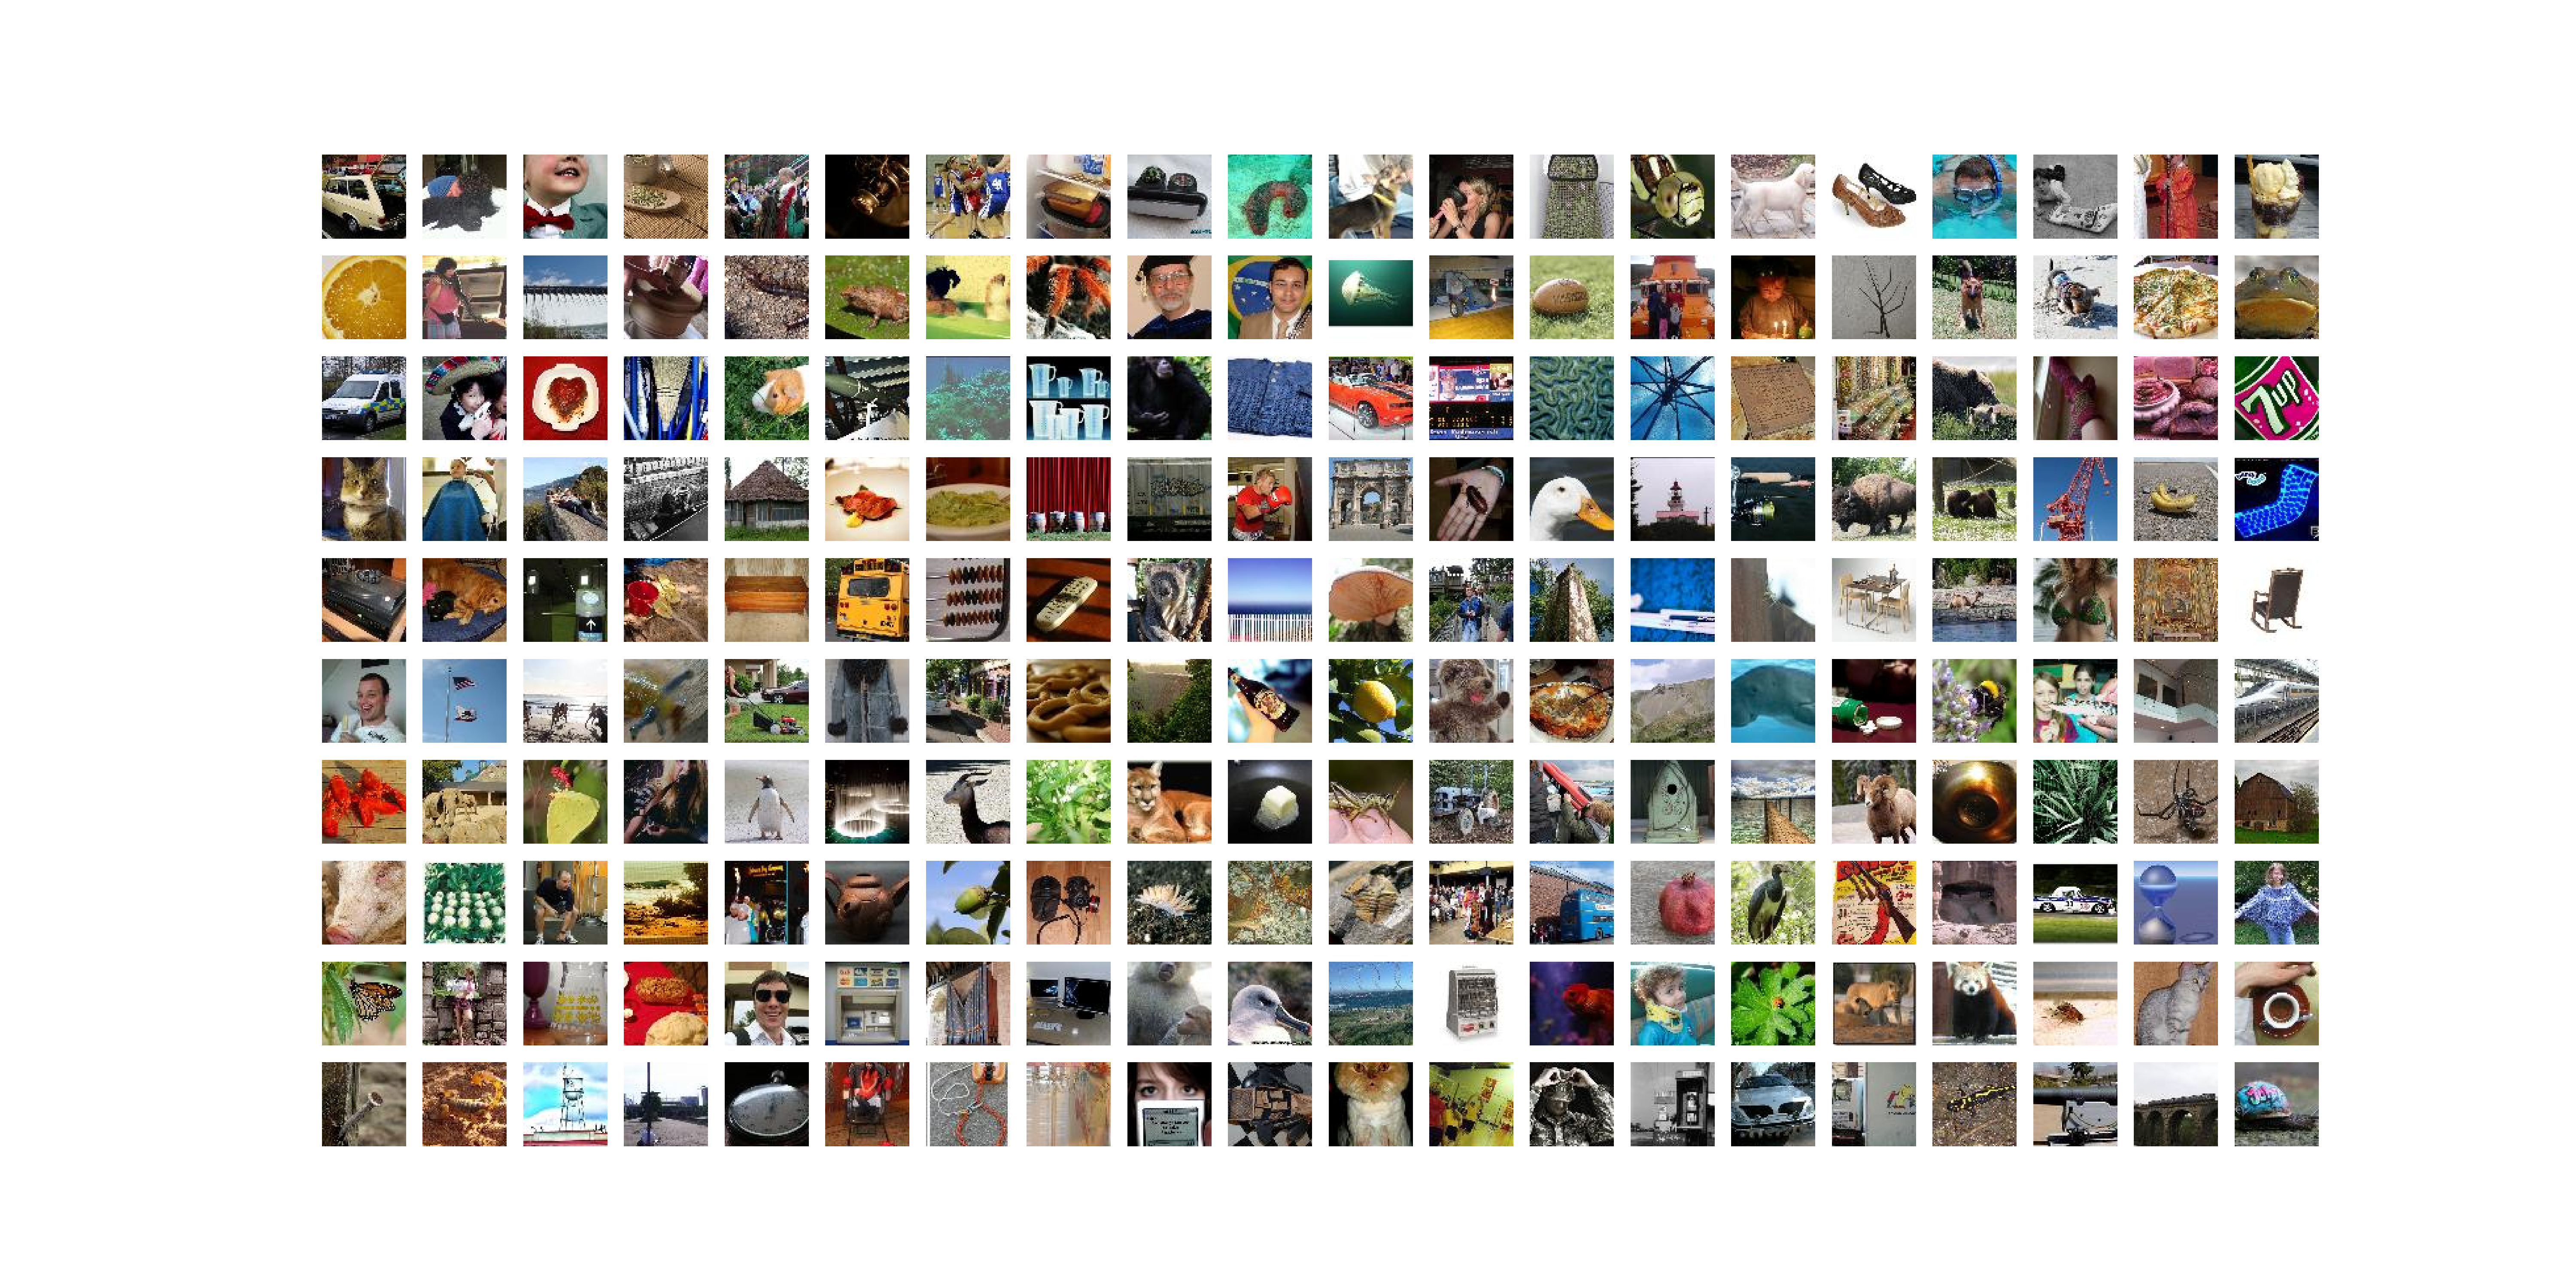
\includegraphics[width=0.9\textwidth]{chapter_dlo/assets/tinyimagenet_example.png}
  \caption{A sample of images from the Tiny ImageNet dataset. Each image
    represents an instance of one of the  200 distinct classes.}
  \label{fig:intro:tinyimagenet_examples}
\end{figure}

\subsection{Train, Validation and Test Sets}

In our experiments, for each dataset, we use 3 distinct sets for training,
validation and testing. The training set serves to tune the weights of the
model, while the validation set is used to monitor the evolution of the
performance metric on unseen data throughout the training. The validation metric
provides the necessary triggers for the early stopping policy (\emph{i.e.}
interrupting the training prematurely if the validation metrics do not change
over a given number of iterations). The test set, on the other hand, is used to
evaluate the model's performance on entirely new data and to report the final
test accuracy. When utilizing datasets like CIFAR-10 and CIFAR-100, only
training and testing sets are available. For these datasets, we split the given
train set using the following proportions: 90\% is used for training the network
and the remaining 10\% is for validation. On the other hand, the TinyImageNet
dataset does provide training, validation, and testing sets, but the test set
lacks annotations. Hence, we use 90\% of the original training set for model
training and the remaining 10\% for validation. Instead of the original
unannotated test set, we repurpose the original validation set to serve as the
test set. This is a common strategy employed by other implementations
\cite{hanyuanxu2018tinyimagenet,nbdt,alvinwan2020nbdt}.\\
